\documentclass[a4paper, 12pt]{extarticle}

% Includes 
\usepackage[utf8]{inputenc} % UTF-8 encode 
\usepackage[english, russian]{babel}
\usepackage{geometry} % adjust page layout 
\usepackage{graphicx} 
\usepackage{hyperref} 
\usepackage{amsmath} % math formulas 
\usepackage{setspace} % for set line spacing 
\usepackage{indentfirst} % indent on a first line after the paragraph 
% \usepackage{pgfplots} % for plots 
\usepackage{listings} % for code listings 
\usepackage{xcolor} % colors (used for listings)
\usepackage{sourcecodepro} % for another monospaced font 
\usepackage{cmap} % for correct search in pdf
\usepackage{placeins} % for \FloatBarrier
\usepackage{subcaption} % for subfigures


% debug
% \usepackage{showframe} % frame borders for demonstration 


%%% Custom commands
% commands for unnumbered sections
\newcommand{\usection}[1]{\section*{#1} \addcontentsline{toc}{section}{\protect\numberline{}#1}}
\newcommand{\usubsection}[1]{\subsection*{#1} \addcontentsline{toc}{subsection}{\protect\numberline{}#1}}
\newcommand{\usubsubsection}[1]{\subsubsection*{#1} \addcontentsline{toc}{subsubsection}{\protect\numberline{}#1}}


% Redefinition of section and subsection numbering style
\def\thesection{\arabic{section}.}
\def\thesubsection{\arabic{section}.\arabic{subsection}.}
\def\thesubsubsection{\arabic{section}.\arabic{subsection}.\arabic{subsubsection}.}


% Settings for links 
\hypersetup{
    colorlinks,
    citecolor=black,
    filecolor=black,
    linkcolor=black,
    urlcolor=black
}


% Layout
\geometry{
	left=17mm,
	top=17mm,
	right=17mm,
	bottom=20mm,
	marginparsep=0mm,
	marginparwidth=0mm,
	headheight=8mm,
	headsep=5mm, 
}

\linespread{1.5} % line spacing
\setlength{\parskip}{\baselineskip}  % Add space between paragraphs


% overfull hbox settings
\tolerance 10000 % default 200, max 10000
\hbadness 10000 % default 1000, max 10000
\emergencystretch 0pt  % default 0pt, how much the lines can stretch for the sake of good line breaks
\hfuzz 0.4pt % ignore overfull box less than 
\widowpenalty=10000 % no lines at the start of the page
\vfuzz \hfuzz % don't care about underfull vbox if overfull is acceptable
\raggedbottom % if the page is not filled, align the content to the bottom


% Redefinition of table of contents command to get centered heading
\makeatletter
\renewcommand\tableofcontents{ 
  \begin{singlespace}
    \null\hfill\textbf{\Large\contentsname}\hfill\null\par
    \@mkboth{\MakeUppercase\contentsname}{\MakeUppercase\contentsname}%
    \@starttoc{toc}
  \end{singlespace}
}
\makeatother


% Listings settings
\definecolor{codegreen}{rgb}{0, 0.6, 0}
\definecolor{codegray}{rgb}{0.5, 0.5, 0.5}
\definecolor{codepurple}{rgb}{0.58, 0, 0.82}
\definecolor{backcolour_gray}{rgb}{0.98, 0.98, 0.98}

\lstdefinestyle{python_white}{
  language=Python,
  backgroundcolor=\color{backcolour_gray},   
  commentstyle=\color{codegreen},
  keywordstyle=\color{blue},
  numberstyle=\tiny\color{codegray},
  stringstyle=\color{codepurple},
  basicstyle=\ttfamily\small\singlespacing,
  breakatwhitespace=true,         
  breaklines=true,                 
  captionpos=b, % t/b                  
  keepspaces=true,                 
  numbers=none, % none/left/rigth                    
  numbersep=5pt,                  
  showspaces=false,                
  showstringspaces=false,
  showtabs=false,                  
  tabsize=2,
  frame=single, % none/leftline/topline/bottomline/lines/single/shadowbox
  rulecolor=\color{gray}, % frame color 
}


\lstset{style=python_white}


% For title page
\def\name{Отчет по лабораторной работе №3} 
\def\subname{Фильтрация изображений}
\def\madeby{Александр Иванов, Ф ТЕХ.ЗРЕНИЕ 1.1 \\ Ани Аракелян, ТЕХ.ЗРЕНИЕ 1.1\\ Никита Братушка, ТЕХ.ЗРЕНИЕ 1.3}
\def\teacher{Шаветов С. В.}

\begin{document}

% Title page 
\begin{titlepage}

\thispagestyle{empty}

\title{


\includegraphics[width=4cm]{media/ITMO_logo.png} 

\vspace{1em}
НИУ ИТМО 
\vspace{4em}

\begin{center}
\large\textsc{\textbf{\name}}

\vspace{1em}
``\subname'' 

\end{center}

\vspace{3em}

\begin{flushright}
\normalsize{ 
Выполнили: \\ \textbf{\madeby} 

Преподаватель: \\ \textbf{\teacher} 
}
\end{flushright}	

\vfill

\begin{center}
\small{Санкт-Петербург, \the\year}
\end{center}
}


\author{}
\date{}
\maketitle
\thispagestyle{empty}
\end{titlepage} % Title page

\addtocounter{page}{1} % Inc counter to start from 2 
\tableofcontents % Table of contents
\pagebreak

\section{Типы шумов}

\textbf{Шум} -- разнообразные искажения на цифровых изображениях, обусловленные разного рода помехами.

В данной лабораторной работе мы рассмотрим наиболее распространенные модели шумов на примере воздействия их на изображения \ref{img:source}. 

\begin{figure}[ht!!]
    \centering
    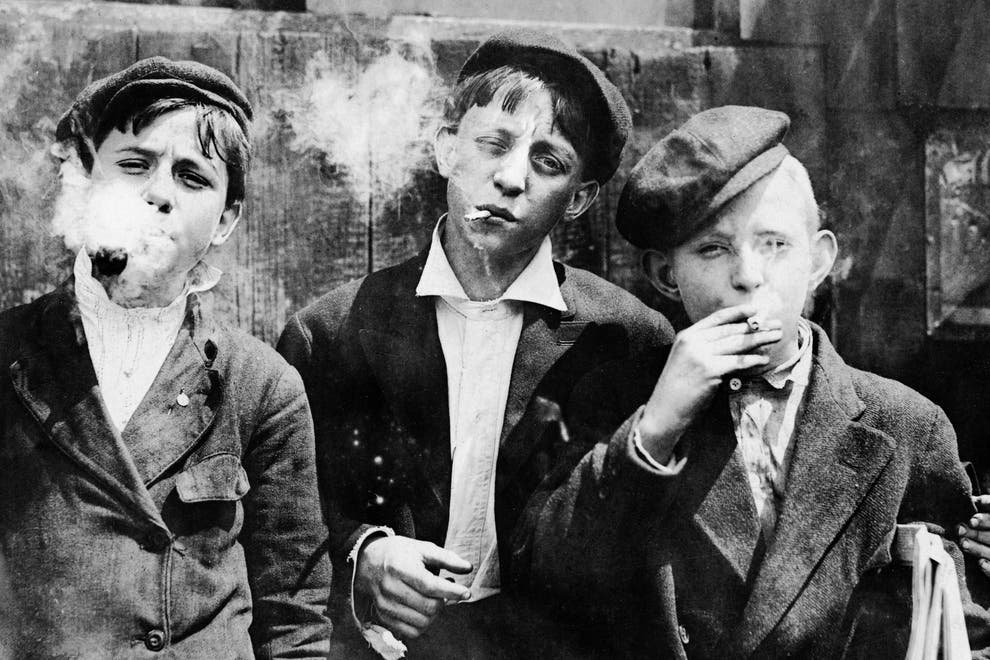
\includegraphics[width=\textwidth]{../lewis-hine-taschen-main-3.jpg}
    \caption{Исходное изображение}
    \label{img:source}  
\end{figure}
\FloatBarrier

\subsection{Импульсный шум}
Зашумленное изображение $I$ описывается следующей системой, причем значение интенсивности пикселя $I(x,y)$ будет изменено на значение $d \in [0,255]$:
\begin{equation}
    \begin{cases} d,\, \text{c вероятностью}\, p, \\
    s_{x,y},\, \text{c вероятностью}\, (1-p),
    \end{cases}
\end{equation}

где $s_{x,y}$ — интенсивность пикселя исходного изображения, если $d = 0$ — шум типа «перец», если
$d = 255$ — шум типа «соль».

\begin{figure}[ht!!]
    \centering
    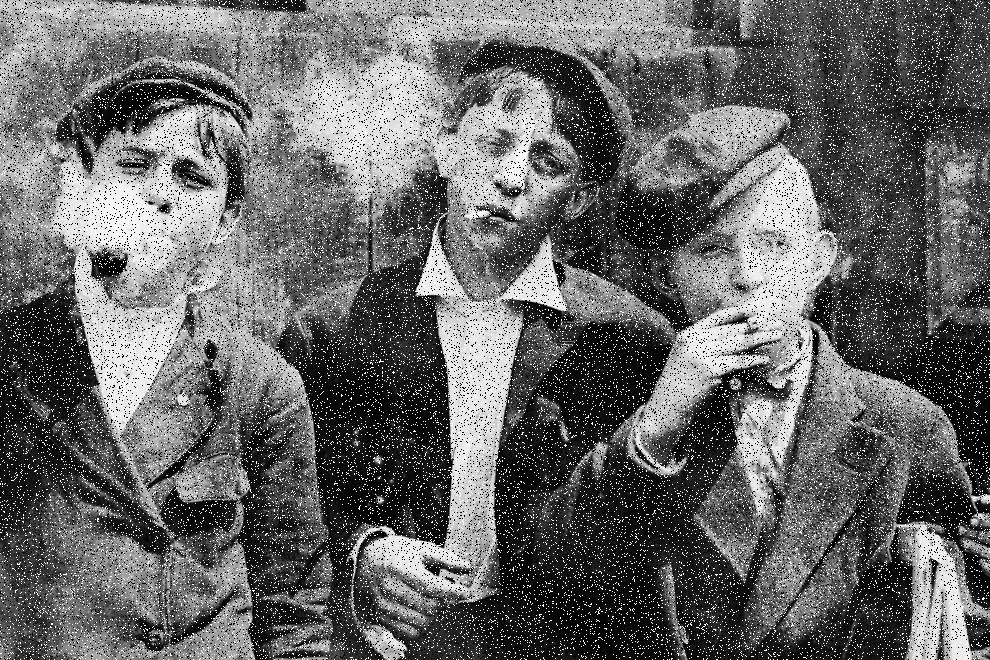
\includegraphics[width=\textwidth]{../Noisy_images/Impulse_noise.jpg}
    \caption{Результат воздействия импульсного шума на изображение \ref{img:source}}
    \label{img:impulse_noise}  
\end{figure}
\FloatBarrier

Итак, на изображении \ref{img:impulse_noise} отчетливо видны появившиеся белые («соль») и черные («перец») точки, что является характерным для импульсного шума, именно из-за этого он часто называется точечным шумом

\subsection{Аддитивный шум}
Аддитивный шум описывается следующим выражением:
\begin{equation}
    I_{new}(x,y) = I(x,y)  + \eta(x,y),
\end{equation}
где $ I_{new}$ — зашумленное изображение, $I$ — исходное изображение, $\eta$ — не зависящий от сигнала аддитивный шум с гауссовым или любым другим распределением функции плотности вероятности.

\begin{figure}[ht!!]
    \centering
    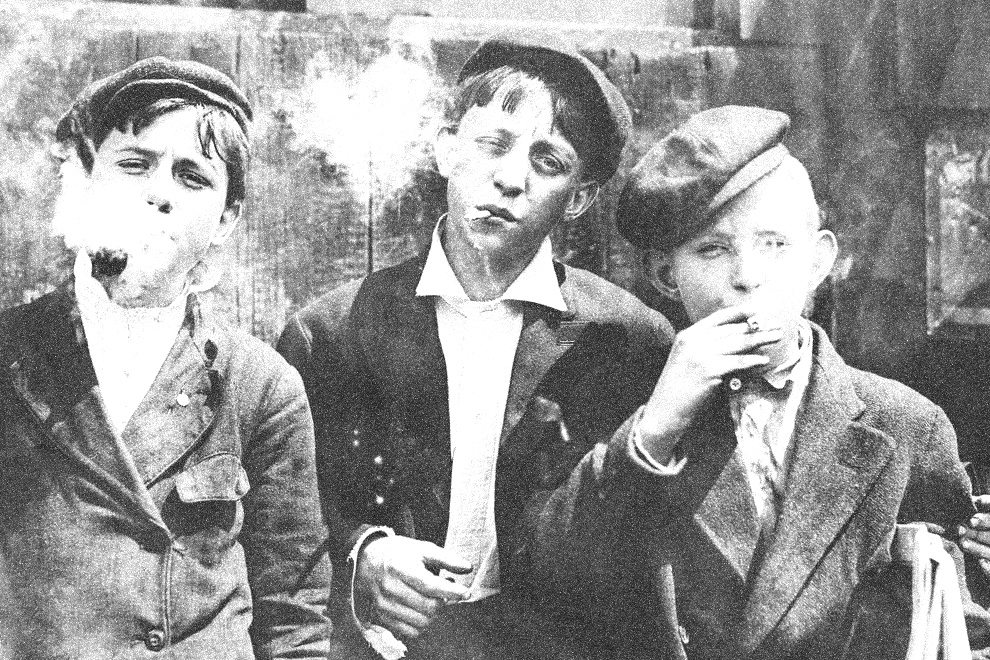
\includegraphics[width=\textwidth]{../Noisy_images/Additive_noise.jpg}
    \caption{Результат воздействия аддитивного шума на изображение \ref{img:source}}
    \label{img:additive_noise}
\end{figure}
\FloatBarrier

Наложив аддитивный шум на исходное изображение, мы получили как будто выцветшую картинку, на которой также появилась небольшая зернистость

\subsection{Мультипликативный шум}
Мультипликативный шум описывается следующим выражением:
\begin{equation}
    I_{new}(x,y) = I(x,y) \cdot \eta(x,y),
\end{equation}

Частным случаем мультипликативного шума является спекл-шум, который мы и рассмотрим

\begin{figure}[ht!!]
    \centering
    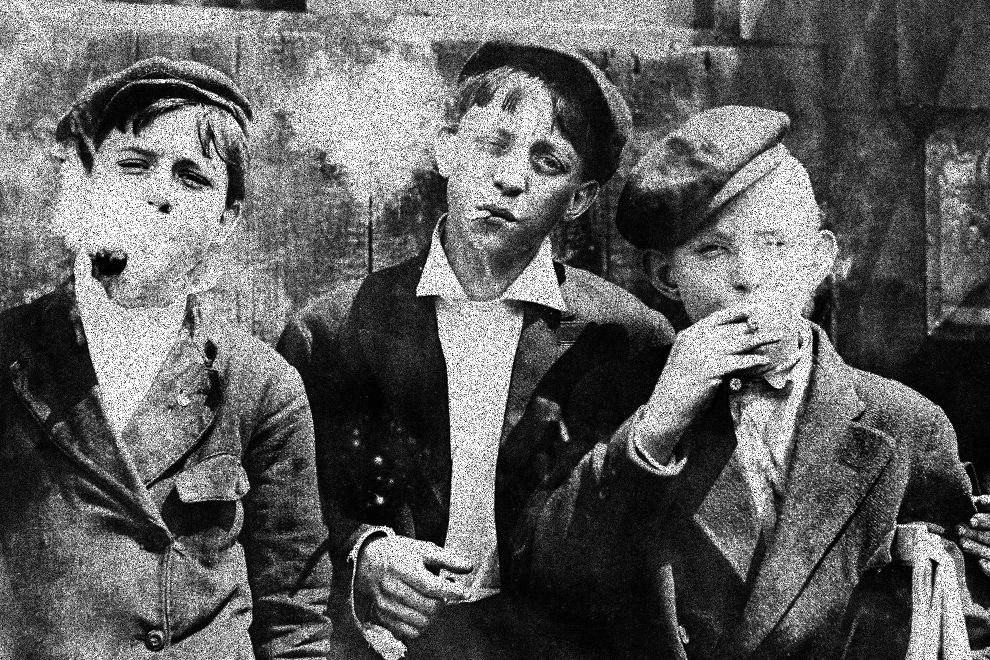
\includegraphics[width=\textwidth]{../Noisy_images/Speckle_noise.jpg}
    \caption{Результат воздействия спекл-шума на изображение \ref{img:source}}
    \label{img:speckle_noise}
\end{figure}
\FloatBarrier

Мы получили изображение на котором можно отчетливо наблюдать светлые пятна, крапинки (спеклы), которые разделены темными участками изображения, что соответственно характерно при наложении спекл-шума

\subsection{Гауссов (нормальный) шум}
Функция распределения плотности вероятности
$p(z)$ случайной величины $z$ описывается следующим выражением:
\begin{equation}
    p(z)= \frac{1}{\sigma\sqrt{2\pi}}\, e^{\frac{-(z-\mu)^2}{2\sigma^2}},
\end{equation}
где $z$ — интенсивность изображения (например, для полутонового изображения $z \in [0,255]$), $\eta$ — среднее (математическое ожидание) случайной величины $z$, $\sigma$ — среднеквадратичное отклонение, дисперсия $\sigma^2$ определяет мощность вносимого шума.


\begin{figure}[ht!!]
    \centering
    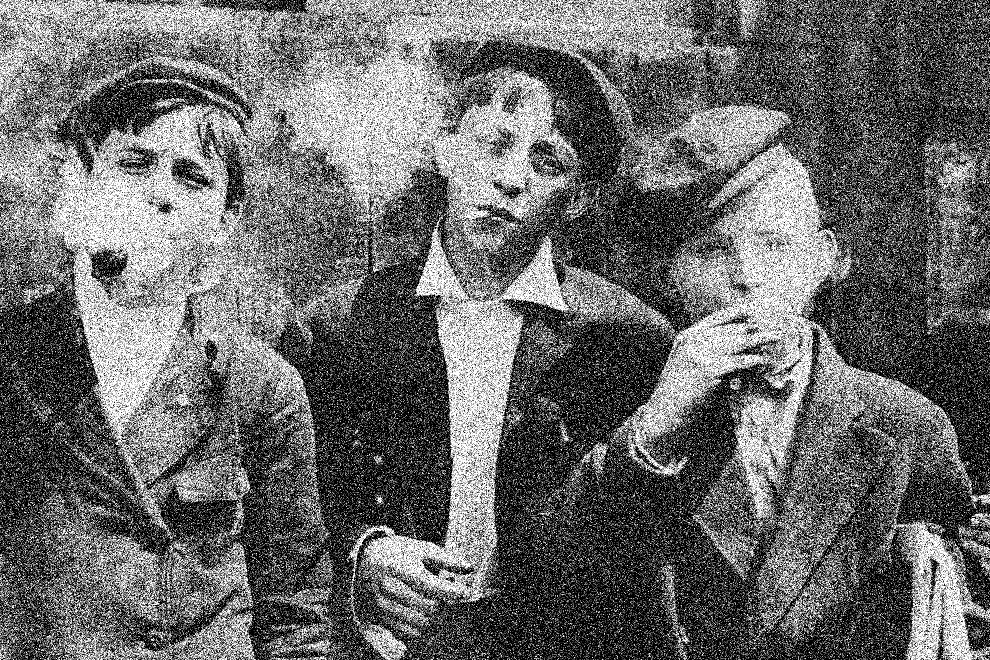
\includegraphics[width=\textwidth]{../Noisy_images/Gaussian_noise.jpg}
    \caption{Результат воздействия Гауссова шума на изображение \ref{img:source}}
    \label{img:gaussian_noise}
\end{figure}
\FloatBarrier

При применении Гауссового (нормального) шума к изображению, оно становится более размытым или зернистым. Он добавляет случайные значения пикселям изображения, что приводит к потере деталей и четкости.

\subsection{Шум квантования}
Приближенно шум квантования можно описать распределением Пуассона. Такой шум не устраняется.

\begin{figure}[ht!!]
    \centering
    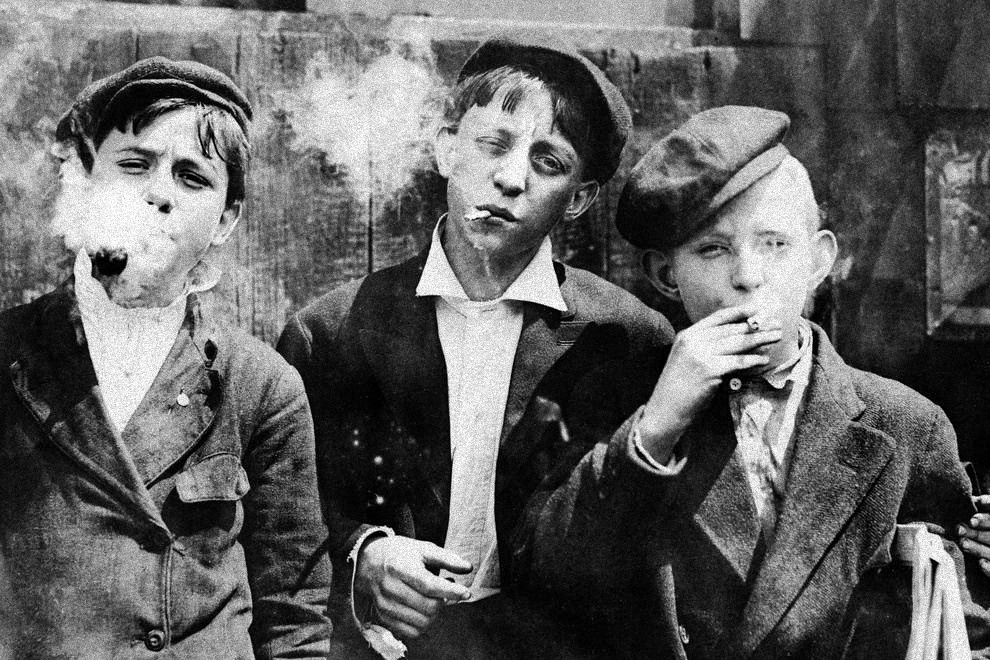
\includegraphics[width=\textwidth]{../Noisy_images/Poisson_Noise.jpg}
    \caption{Результат воздействия шума квантования на изображение \ref{img:source}}
    \label{img:poisson_noise}
\end{figure}
\FloatBarrier

Шум на первый взгляд может показаться незаметным, но он есть, при сильном растяжении изображения это видно. На картинке появилась очень мелкая зернистость

\section{Фильтрация изображений}
\textit{Локальным} преобразованием называется такое преобразование, при котором для вычисления значения интенсивности каждого пикселя учитываются значения соседних пикселей в некоторой окрестности, называемой \textit{окном}, представляющей собой некоторую матрицу, которую также называют \textit{маской, фильтром, ядром фильтра}, а сами значения элементов
матрицы соответсвенно \textit{коэффициентами}. Как правило, маска имеет квадратную форму.

Фильтрация изображения $I$, имеющего размеры $M \times N$, с помощью маски размера $m \times n$ описывается формулой:
\begin{equation}
    I_{new}(x,y) = \sum_s \sum_t w(s,t) I(x+s,y+t),
\end{equation}
где $s$ и $t$ — координаты элементов маски относительно ее центра (в
центре $s = t = 0$). Такого рода преобразования называются \textit{линейными}.

\textit{Фильтрация в скользящем окне} — преобразование, при котором после вычисления нового значения интенсивности пикселя $I_{new}(x,y)$ окно $w$, в котором описана маска фильтра, сдвигается и
вычисляется интенсивность следующего пикселя.

\subsection{Низкочастотная фильтрация}
Низкочастотные пространственные фильтры ослабляют высокочастотные компоненты (области с сильным изменением интенсивностей) и оставляют низкочастотные компоненты изображения
без изменений. Отличительными особенностями
ядра низкочастотного фильтра являются: неотрицательные коэффициенты маски и то, что сумма всех коэффициентов равна единице.

\subsubsection{Контргармонический усредняющий фильтр}
Фильтр базируется на выражении:
\begin{equation}
    I_{new}(x,y) = \frac{\sum_{i=0}^m \sum_{j=0}^n I(i,j)^{Q+1}}{\sum_{i=0}^m \sum_{j=0}^n I(i,j)^Q}, \: \text{где $Q$ — порядок фильтра.}
\end{equation}


Рассмотрим применение фильтра при $Q > 0$ и $Q < 0$ к различным типам шумов. 

\begin{figure}[ht!] 
    \centering
    \begin{subfigure}[b]{0.5\linewidth}
        \centering
        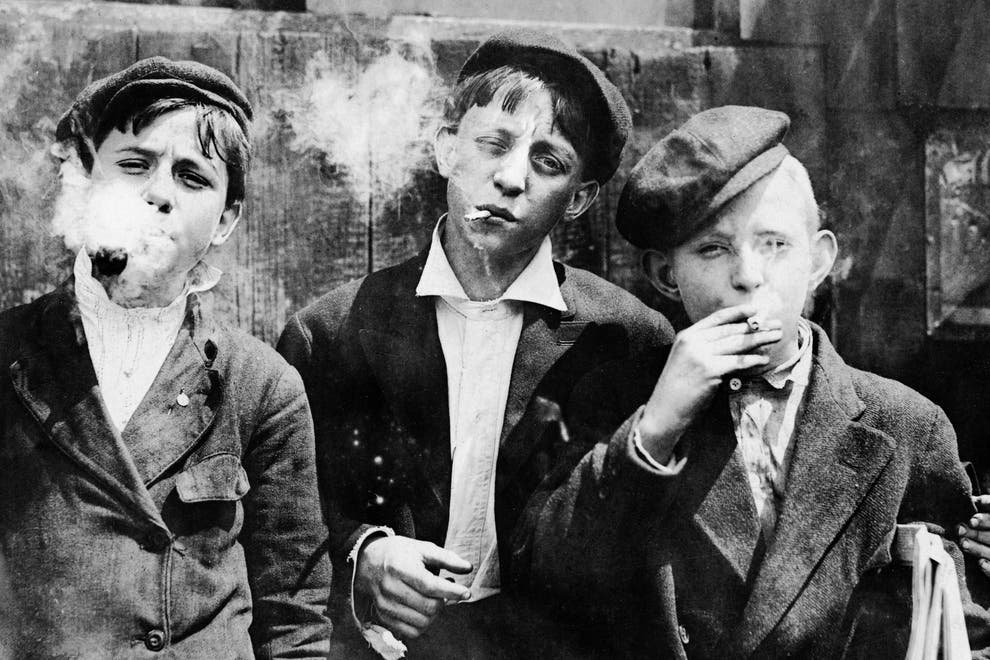
\includegraphics[width=0.95\linewidth]{../lewis-hine-taschen-main-3.jpg} 
        \caption{Исходное изображение} 
        \label{contraharmonic_-1.85:a} 
        \vspace{4ex}
    \end{subfigure}%%
    \begin{subfigure}[b]{0.5\linewidth}
      \centering
      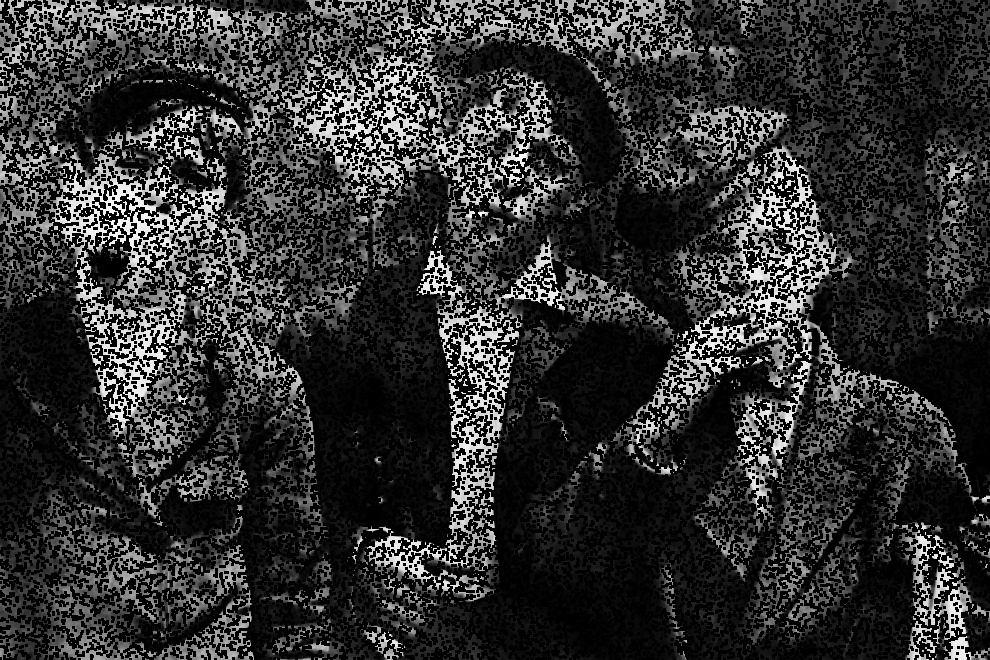
\includegraphics[width=0.95\linewidth]{../Contraharmonic_Filter/Contraharmonic_Impulse_noise_(m,n=(3,_3),q=-1.85).jpg} 
      \caption{Импульсный шум} 
      \label{contraharmonic_-1.85:b} 
      \vspace{4ex}
    \end{subfigure}
    \begin{subfigure}[b]{0.5\linewidth}
      \centering
      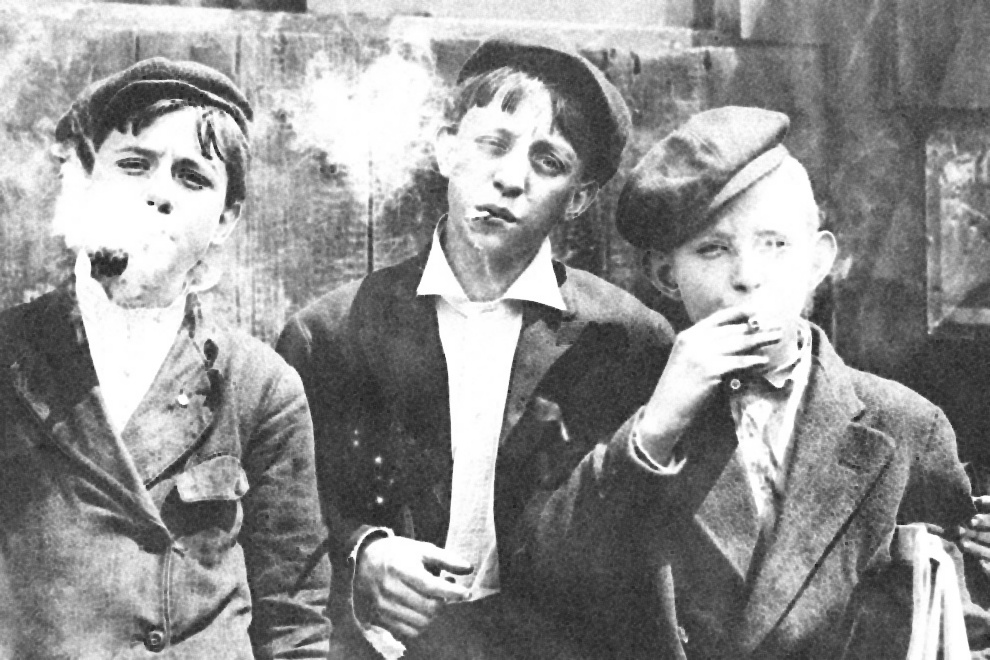
\includegraphics[width=0.95\linewidth]{../Contraharmonic_Filter/Contraharmonic_Additive_noise_(m,n=(3,_3),q=-1.85).jpg} 
      \caption{Аддитивный шум} 
      \label{contraharmonic_-1.85:c} 
      \vspace{4ex}
    \end{subfigure}%%
    \begin{subfigure}[b]{0.5\linewidth}
      \centering
      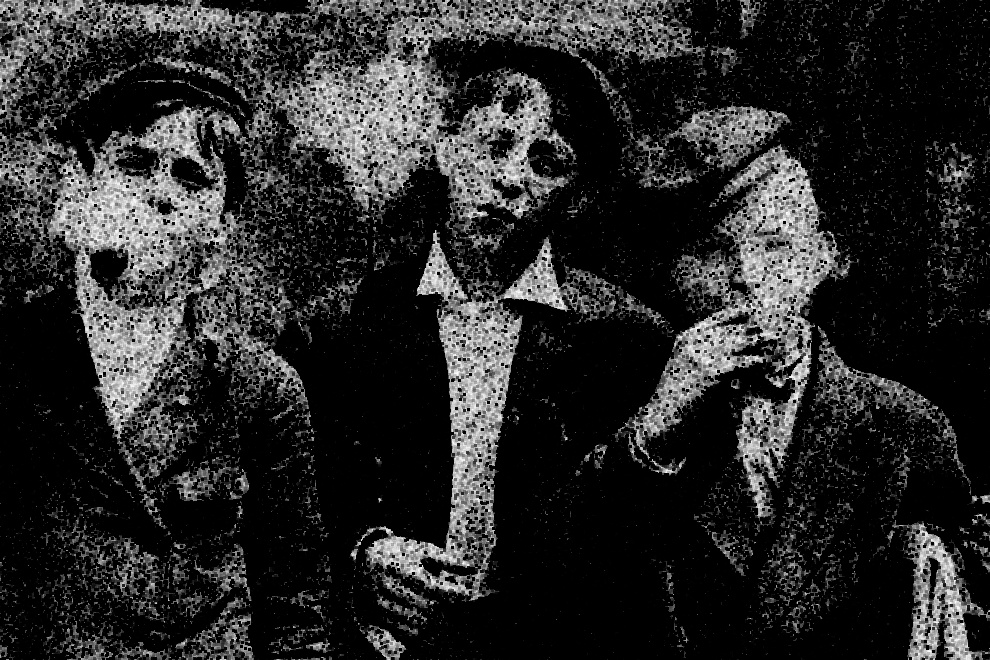
\includegraphics[width=0.95\linewidth]{../Contraharmonic_Filter/Contraharmonic_Gaussian_noise_(m,n=(3,_3),q=-1.85).jpg} 
      \caption{Гауссов шум} 
      \label{contraharmonic_-1.85:d} 
      \vspace{4ex}
    \end{subfigure}
    \begin{subfigure}[b]{0.5\linewidth}
      \centering
      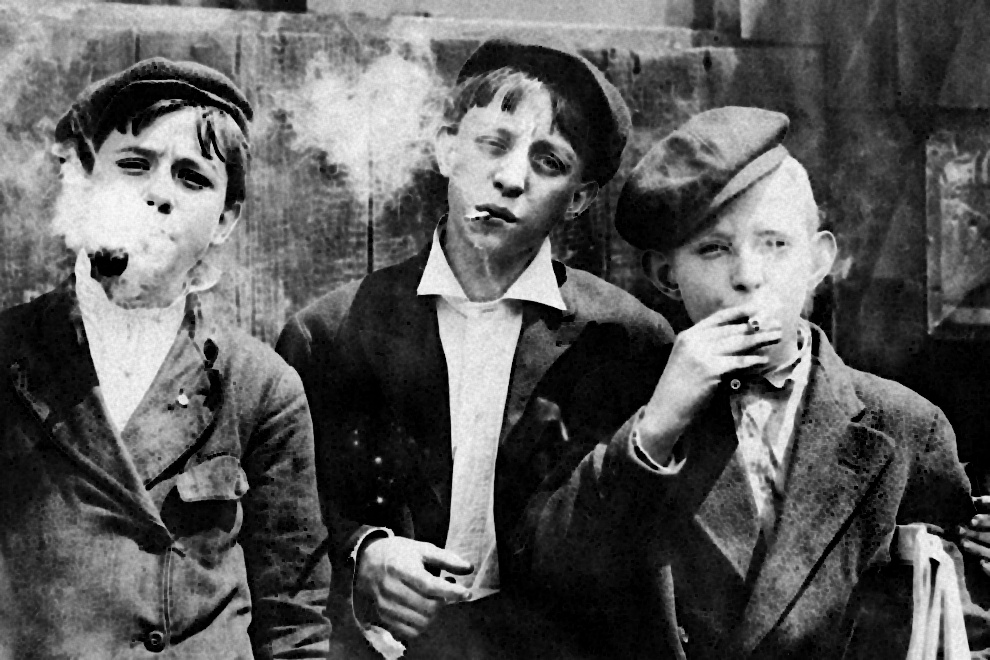
\includegraphics[width=0.95\linewidth]{../Contraharmonic_Filter/Contraharmonic_Poisson_noise_(m,n=(3,_3),q=-1.85).jpg} 
      \caption{Шум квантования} 
      \label{contraharmonic_-1.85:e}
    \end{subfigure}%% 
    \begin{subfigure}[b]{0.5\linewidth}
        \centering
        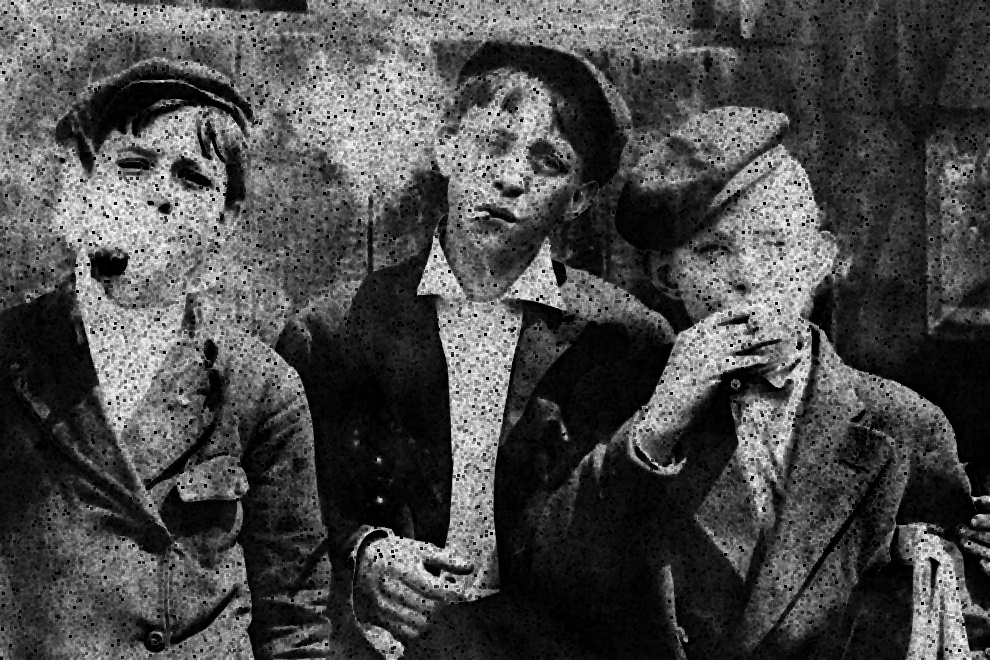
\includegraphics[width=0.95\linewidth]{../Contraharmonic_Filter/Contraharmonic_Speckle_noise_(m,n=(3,_3),q=-1.85).jpg} 
        \caption{Мультипликативный шум} 
        \label{contraharmonic_-1.85:f} 
    \end{subfigure} 
    \caption{Результат применения контргармонического усредняющего фильтра при значении $Q = -1.85$ к различным типам шумов}
    \label{img:contraharmonic_-1.85} 
  \end{figure}

  \begin{figure}[ht!] 
    \centering
    \begin{subfigure}[b]{0.5\linewidth}
        \centering
        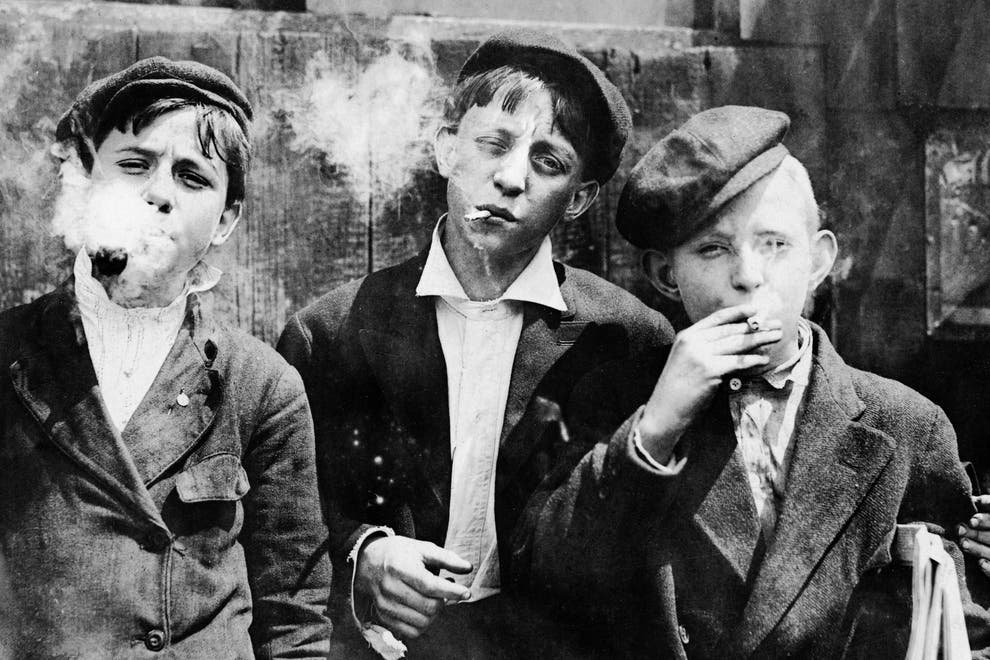
\includegraphics[width=0.95\linewidth]{../lewis-hine-taschen-main-3.jpg} 
        \caption{Исходное изображение} 
        \label{contraharmonic_-0.85:a} 
        \vspace{4ex}
    \end{subfigure}%%
    \begin{subfigure}[b]{0.5\linewidth}
      \centering
      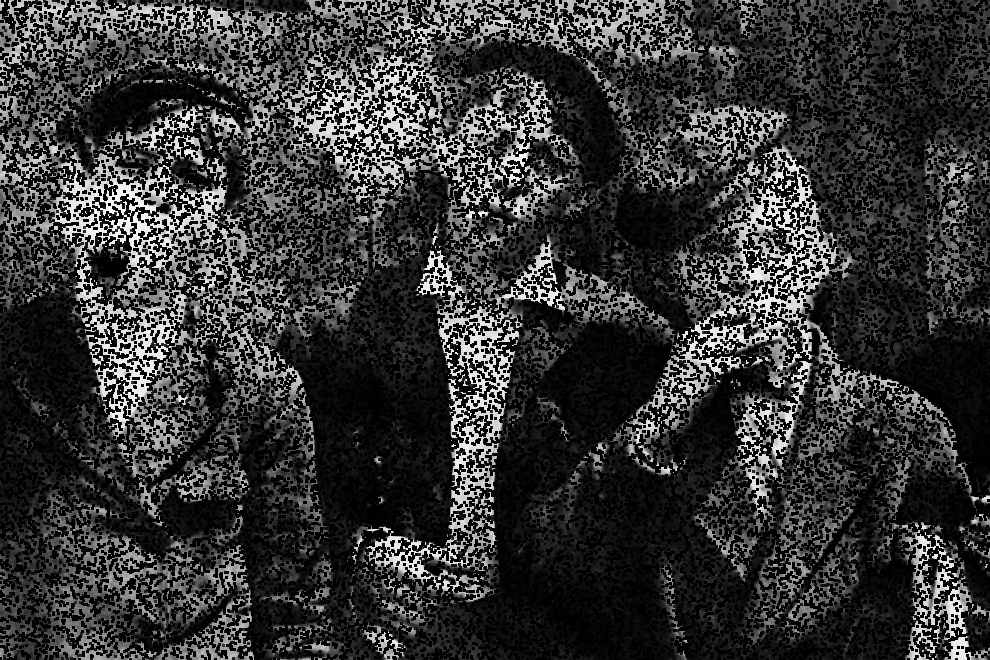
\includegraphics[width=0.95\linewidth]{../Contraharmonic_Filter/Contraharmonic_Impulse_noise_(m,n=(3,_3),q=-0.85).jpg} 
      \caption{Импульсный шум} 
      \label{contraharmonic_-0.85:b} 
      \vspace{4ex}
    \end{subfigure}
    \begin{subfigure}[b]{0.5\linewidth}
      \centering
      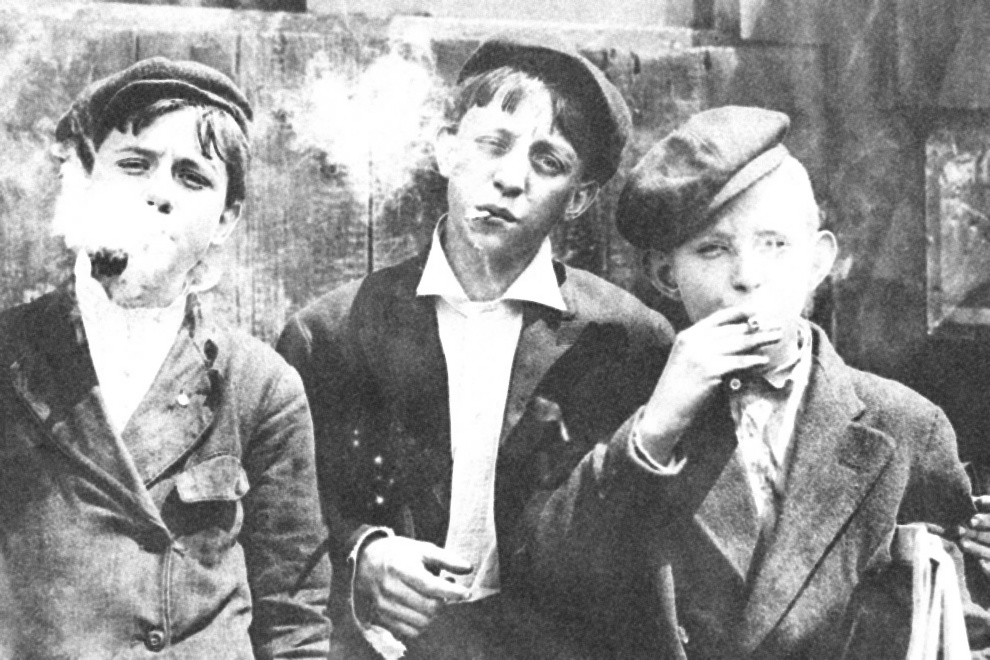
\includegraphics[width=0.95\linewidth]{../Contraharmonic_Filter/Contraharmonic_Additive_noise_(m,n=(3,_3),q=-0.85).jpg} 
      \caption{Аддитивный шум} 
      \label{contraharmonic_-0.85:c} 
      \vspace{4ex}
    \end{subfigure}%%
    \begin{subfigure}[b]{0.5\linewidth}
      \centering
      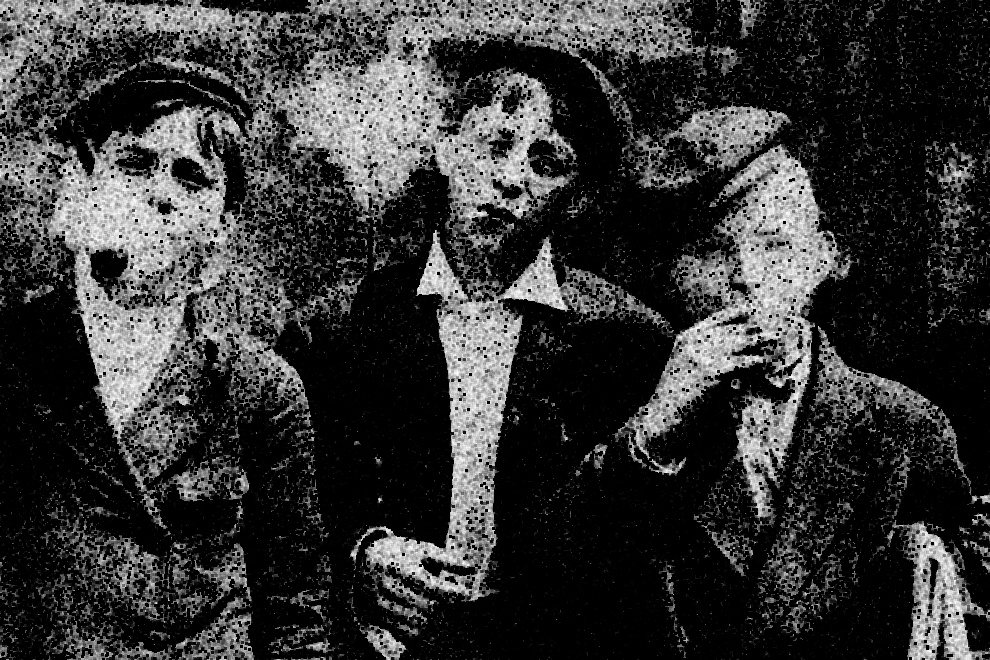
\includegraphics[width=0.95\linewidth]{../Contraharmonic_Filter/Contraharmonic_Gaussian_noise_(m,n=(3,_3),q=-0.85).jpg} 
      \caption{Гауссов шум} 
      \label{contraharmonic_-0.85:d} 
      \vspace{4ex}
    \end{subfigure}
    \begin{subfigure}[b]{0.5\linewidth}
      \centering
      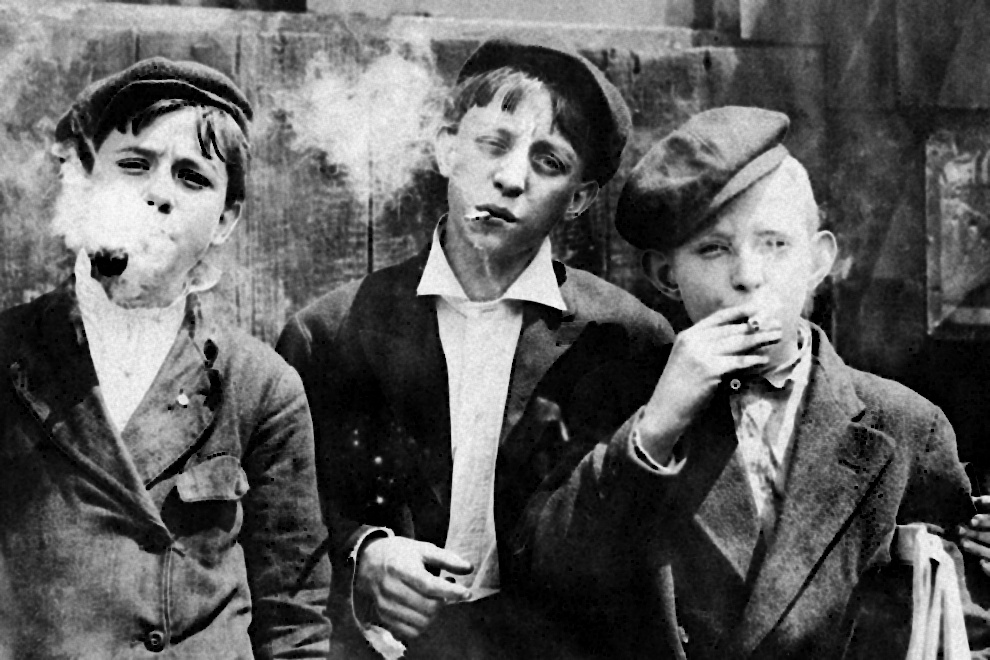
\includegraphics[width=0.95\linewidth]{../Contraharmonic_Filter/Contraharmonic_Poisson_noise_(m,n=(3,_3),q=-0.85).jpg} 
      \caption{Шум квантования} 
      \label{contraharmonic_-0.85:e}
    \end{subfigure}%% 
    \begin{subfigure}[b]{0.5\linewidth}
        \centering
        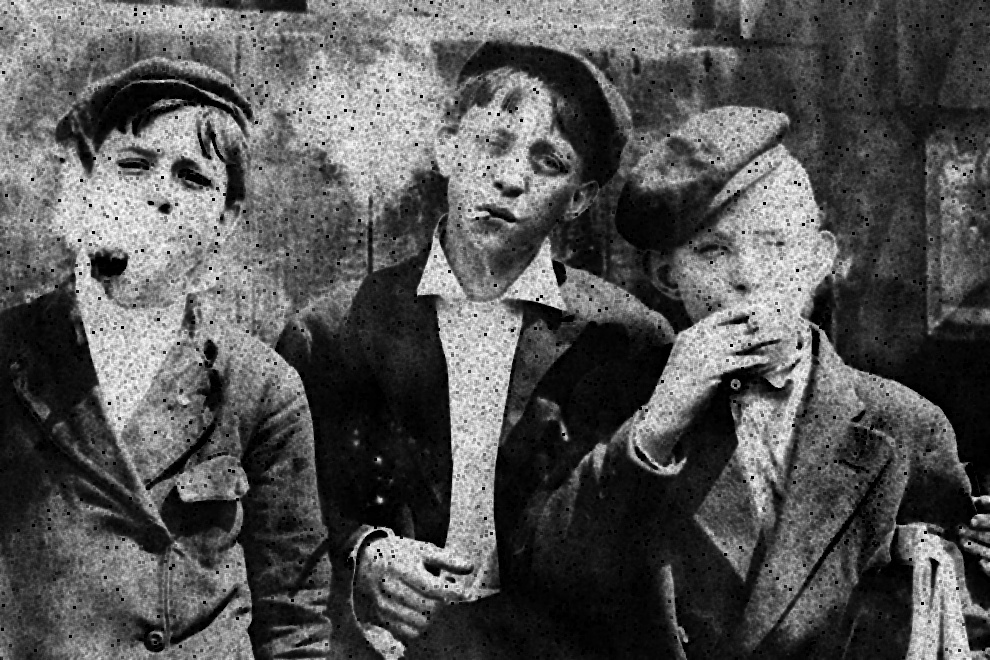
\includegraphics[width=0.95\linewidth]{../Contraharmonic_Filter/Contraharmonic_Speckle_noise_(m,n=(3,_3),q=-0.85).jpg} 
        \caption{Мультипликативный шум} 
        \label{contraharmonic_-0.85:f} 
    \end{subfigure} 
    \caption{Результат применения контргармонического усредняющего фильтра при значении $Q = -0.85$ к различным типам шумов}
    \label{img:contraharmonic_-0.85} 
  \end{figure}

  \begin{figure}[ht!] 
    \centering
    \begin{subfigure}[b]{0.5\linewidth}
        \centering
        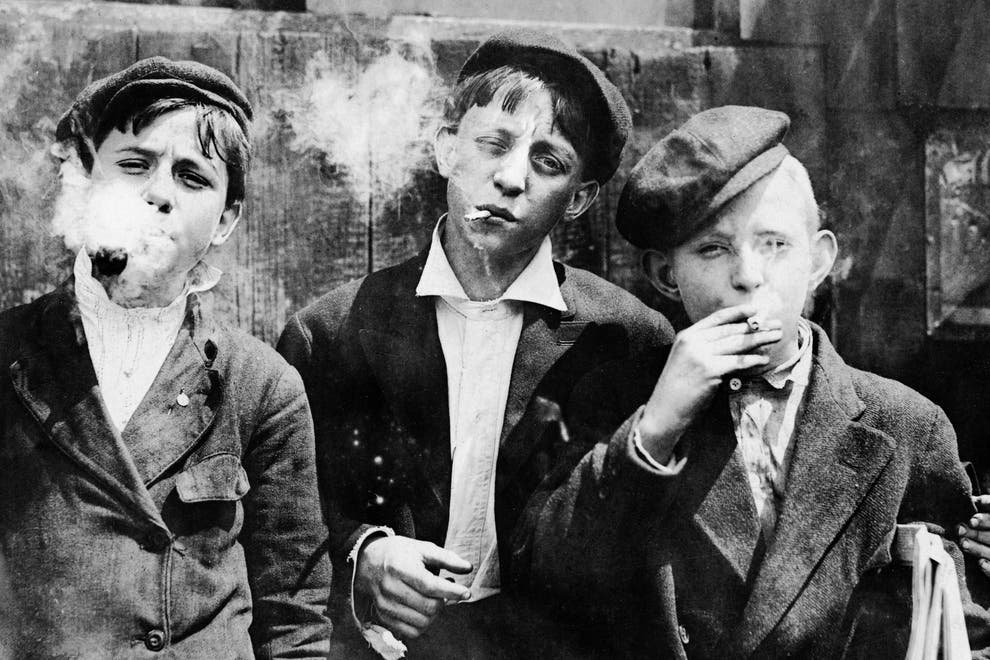
\includegraphics[width=0.95\linewidth]{../lewis-hine-taschen-main-3.jpg} 
        \caption{Исходное изображение} 
        \label{contraharmonic_-0.5:a} 
        \vspace{4ex}
    \end{subfigure}%%
    \begin{subfigure}[b]{0.5\linewidth}
      \centering
      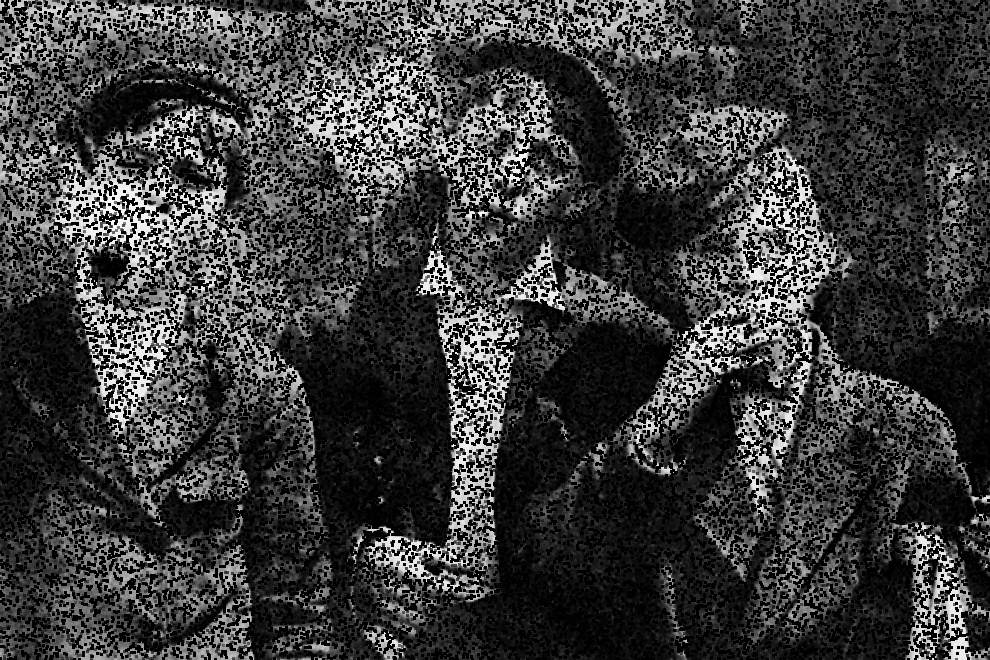
\includegraphics[width=0.95\linewidth]{../Contraharmonic_Filter/Contraharmonic_Impulse_noise_(m,n=(3,_3),q=-0.5).jpg} 
      \caption{Импульсный шум} 
      \label{contraharmonic_-0.5:b} 
      \vspace{4ex}
    \end{subfigure}
    \begin{subfigure}[b]{0.5\linewidth}
      \centering
      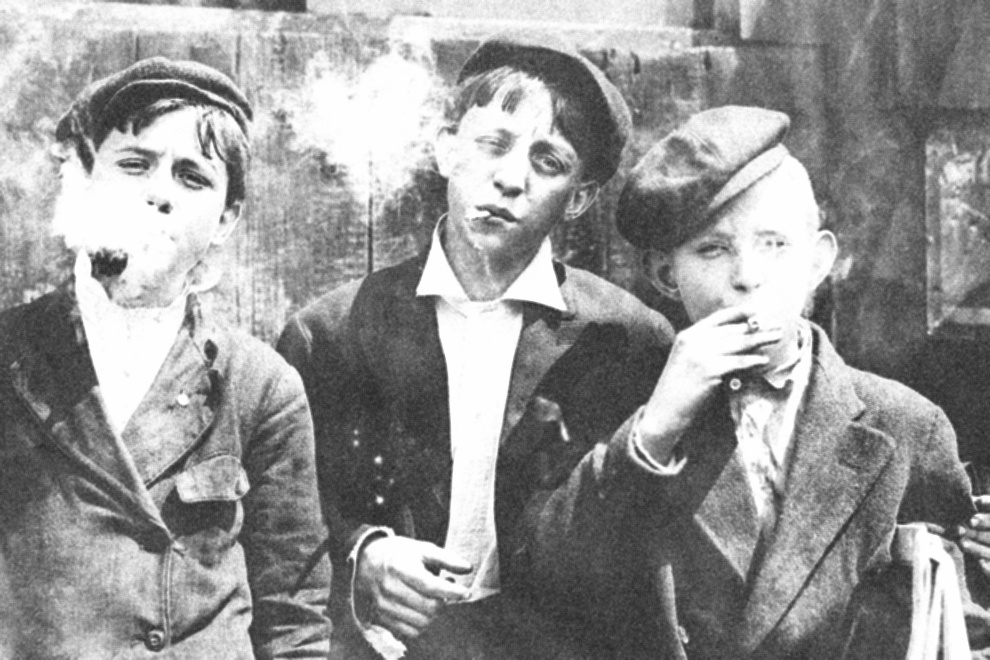
\includegraphics[width=0.95\linewidth]{../Contraharmonic_Filter/Contraharmonic_Additive_noise_(m,n=(3,_3),q=-0.5).jpg} 
      \caption{Аддитивный шум} 
      \label{contraharmonic_-0.5:c} 
      \vspace{4ex}
    \end{subfigure}%%
    \begin{subfigure}[b]{0.5\linewidth}
      \centering
      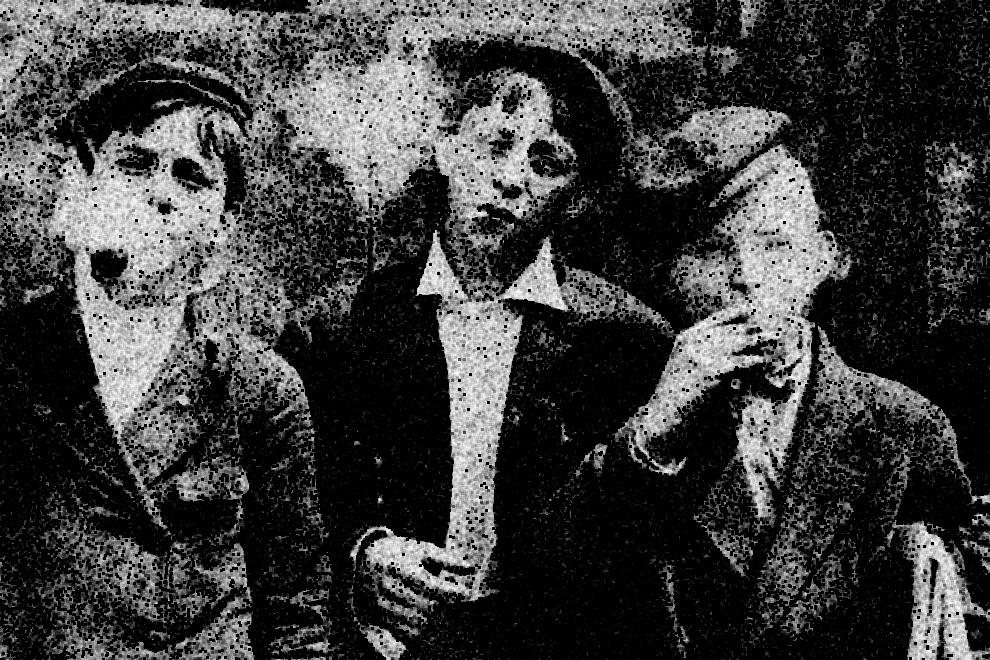
\includegraphics[width=0.95\linewidth]{../Contraharmonic_Filter/Contraharmonic_Gaussian_noise_(m,n=(3,_3),q=-0.5).jpg} 
      \caption{Гауссов шум} 
      \label{contraharmonic_-0.5:d} 
      \vspace{4ex}
    \end{subfigure}
    \begin{subfigure}[b]{0.5\linewidth}
      \centering
      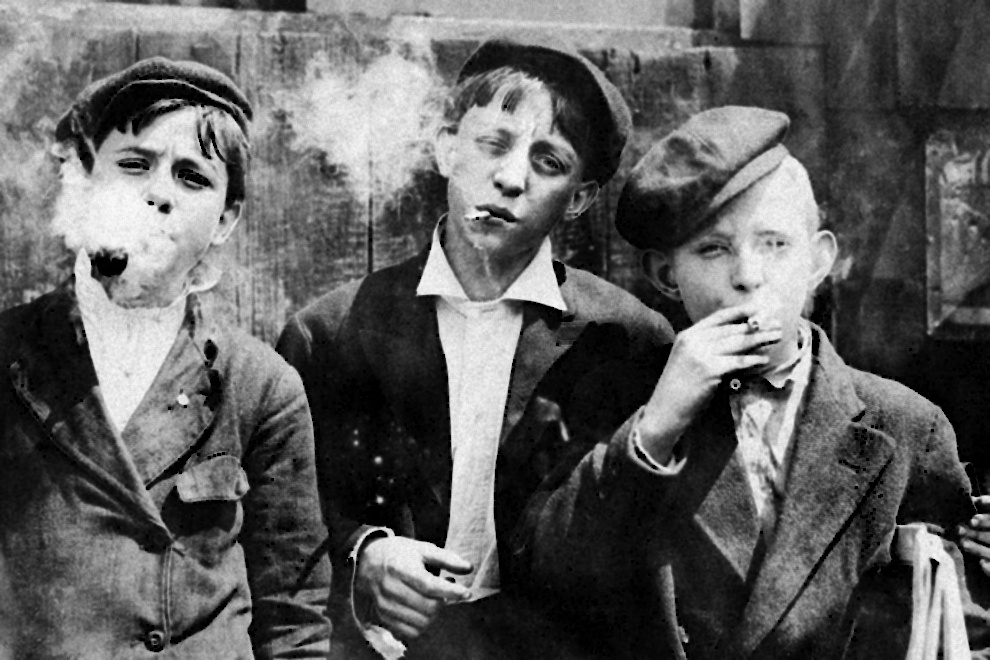
\includegraphics[width=0.95\linewidth]{../Contraharmonic_Filter/Contraharmonic_Poisson_noise_(m,n=(3,_3),q=-0.5).jpg} 
      \caption{Шум квантования} 
      \label{contraharmonic_-0.5:e}
    \end{subfigure}%% 
    \begin{subfigure}[b]{0.5\linewidth}
        \centering
        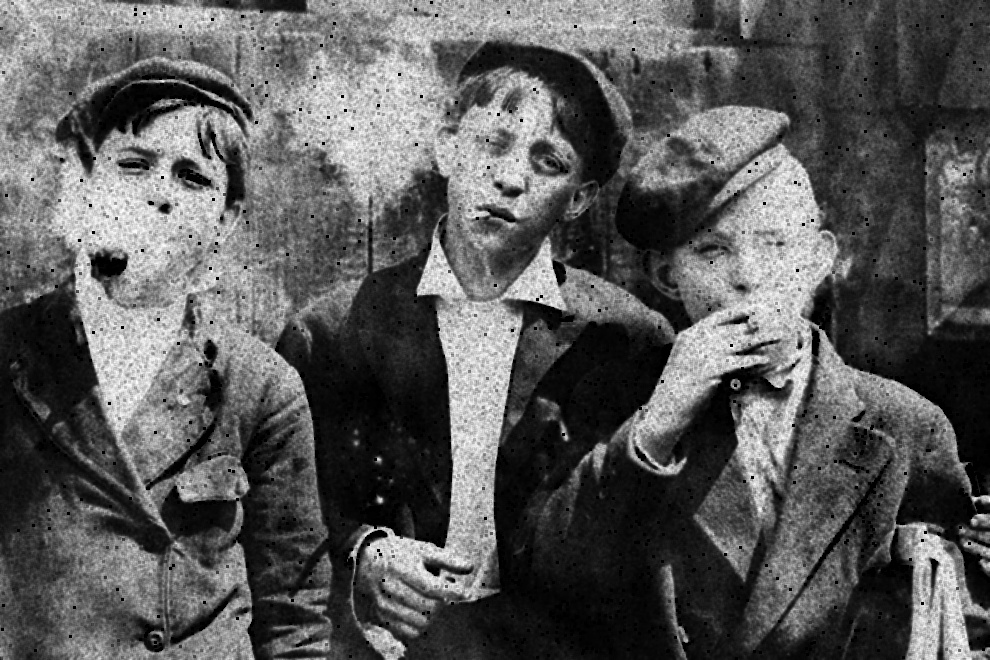
\includegraphics[width=0.95\linewidth]{../Contraharmonic_Filter/Contraharmonic_Speckle_noise_(m,n=(3,_3),q=-0.5).jpg} 
        \caption{Мультипликативный шум} 
        \label{contraharmonic_-0.5:f} 
    \end{subfigure} 
    \caption{Результат применения контргармонического усредняющего фильтра при значении $Q = -0.5$ к различным типам шумов}
    \label{img:contraharmonic_-0.5} 
  \end{figure}

  \begin{figure}[ht!] 
    \centering
    \begin{subfigure}[b]{0.5\linewidth}
        \centering
        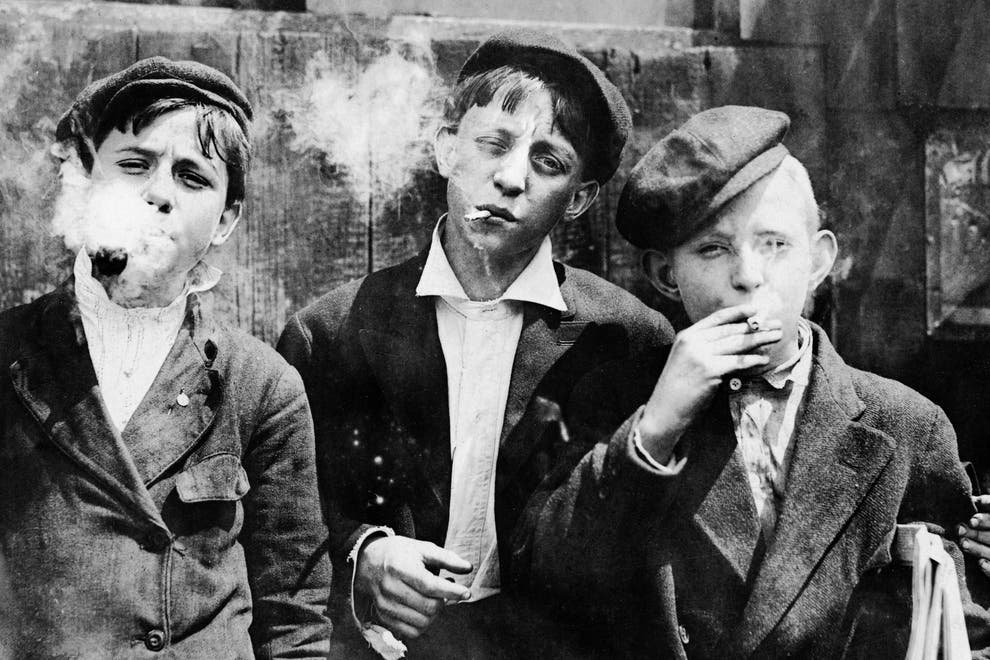
\includegraphics[width=0.95\linewidth]{../lewis-hine-taschen-main-3.jpg} 
        \caption{Исходное изображение} 
        \label{contraharmonic_0.5:a} 
        \vspace{4ex}
    \end{subfigure}%%
    \begin{subfigure}[b]{0.5\linewidth}
      \centering
      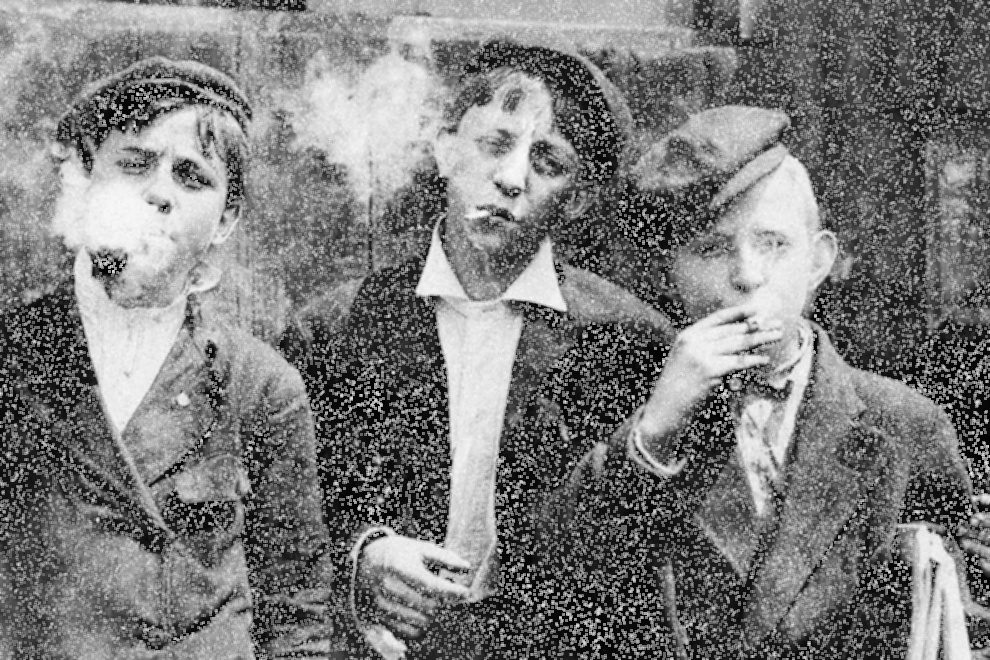
\includegraphics[width=0.95\linewidth]{../Contraharmonic_Filter/Contraharmonic_Impulse_noise_(m,n=(3,_3),q=0.5).jpg} 
      \caption{Импульсный шум} 
      \label{contraharmonic_0.5:b} 
      \vspace{4ex}
    \end{subfigure}
    \begin{subfigure}[b]{0.5\linewidth}
      \centering
      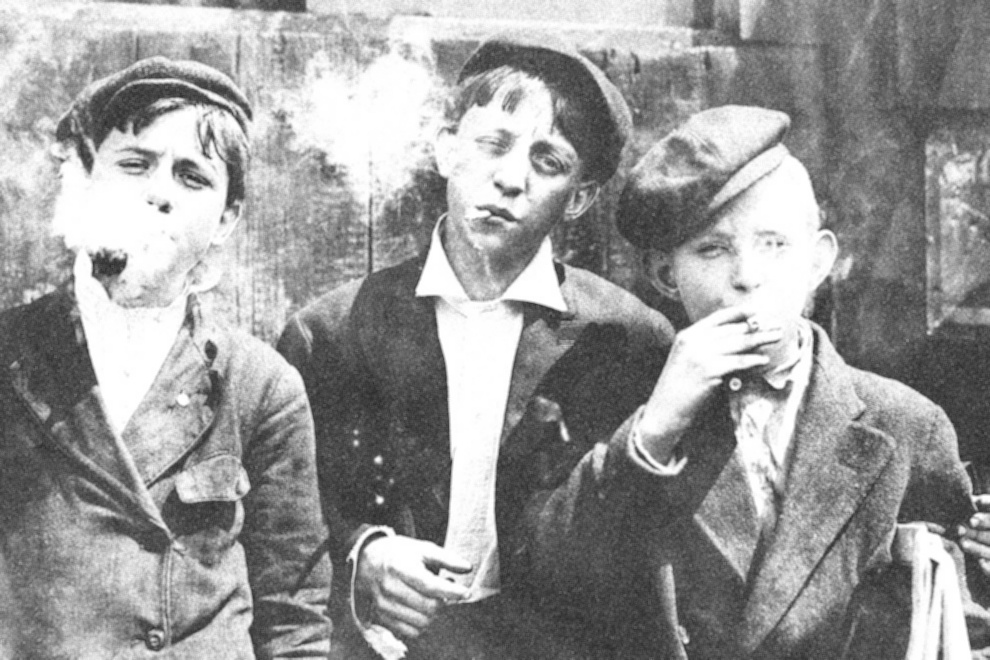
\includegraphics[width=0.95\linewidth]{../Contraharmonic_Filter/Contraharmonic_Additive_noise_(m,n=(3,_3),q=0.5).jpg} 
      \caption{Аддитивный шум} 
      \label{contraharmonic_0.5:c} 
      \vspace{4ex}
    \end{subfigure}%%
    \begin{subfigure}[b]{0.5\linewidth}
      \centering
      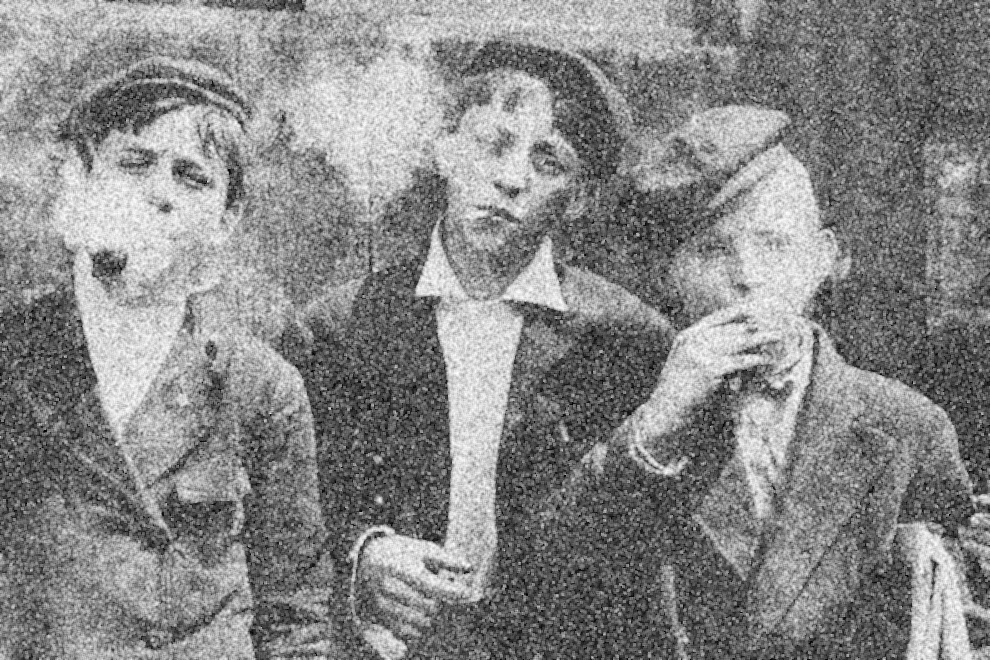
\includegraphics[width=0.95\linewidth]{../Contraharmonic_Filter/Contraharmonic_Gaussian_noise_(m,n=(3,_3),q=0.5).jpg} 
      \caption{Гауссов шум} 
      \label{contraharmonic_0.5:d} 
      \vspace{4ex}
    \end{subfigure}
    \begin{subfigure}[b]{0.5\linewidth}
      \centering
      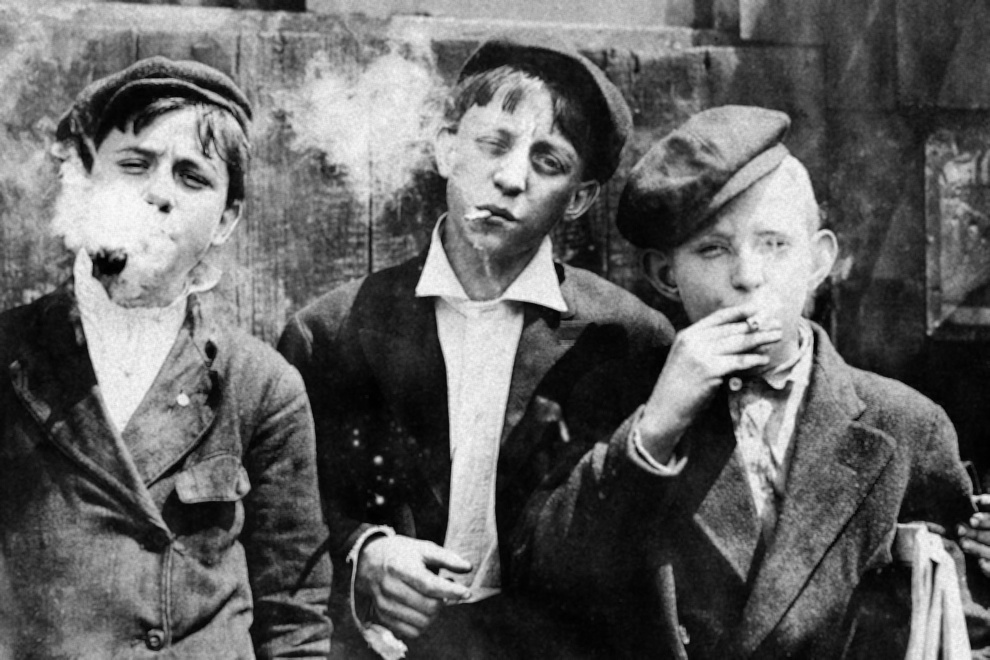
\includegraphics[width=0.95\linewidth]{../Contraharmonic_Filter/Contraharmonic_Poisson_noise_(m,n=(3,_3),q=0.5).jpg} 
      \caption{Шум квантования} 
      \label{contraharmonic_0.5:e}
    \end{subfigure}%% 
    \begin{subfigure}[b]{0.5\linewidth}
        \centering
        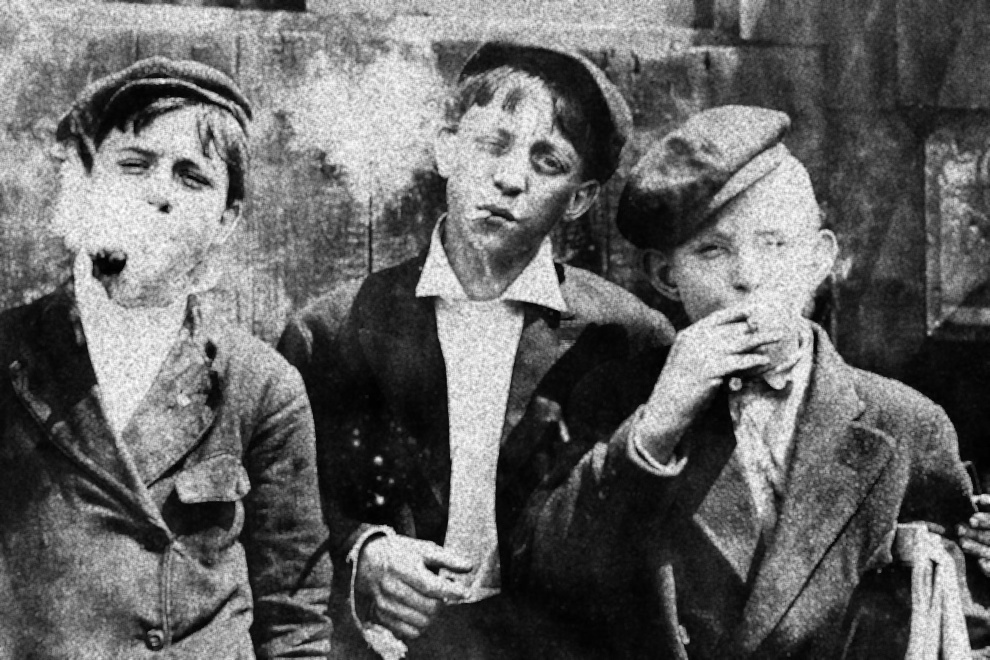
\includegraphics[width=0.95\linewidth]{../Contraharmonic_Filter/Contraharmonic_Speckle_noise_(m,n=(3,_3),q=0.5).jpg} 

        \caption{Мультипликативный шум} 
        \label{contraharmonic_0.5:f} 
    \end{subfigure} 
    \caption{Результат применения контргармонического усредняющего фильтра при значении $Q = 0.5$ к различным типам шумов}
    \label{img:contraharmonic_0.5} 
  \end{figure}

  \begin{figure}[ht!] 
    \centering
    \begin{subfigure}[b]{0.5\linewidth}
        \centering
        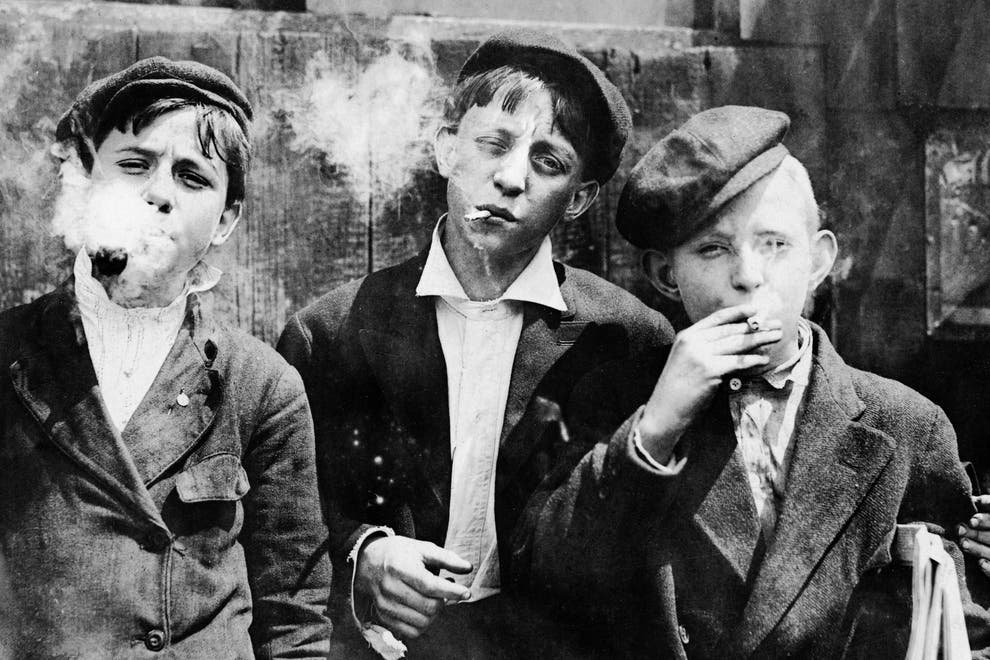
\includegraphics[width=0.95\linewidth]{../lewis-hine-taschen-main-3.jpg} 
        \caption{Исходное изображение} 
        \label{contraharmonic_0.85:a} 
        \vspace{4ex}
    \end{subfigure}%%
    \begin{subfigure}[b]{0.5\linewidth}
      \centering
      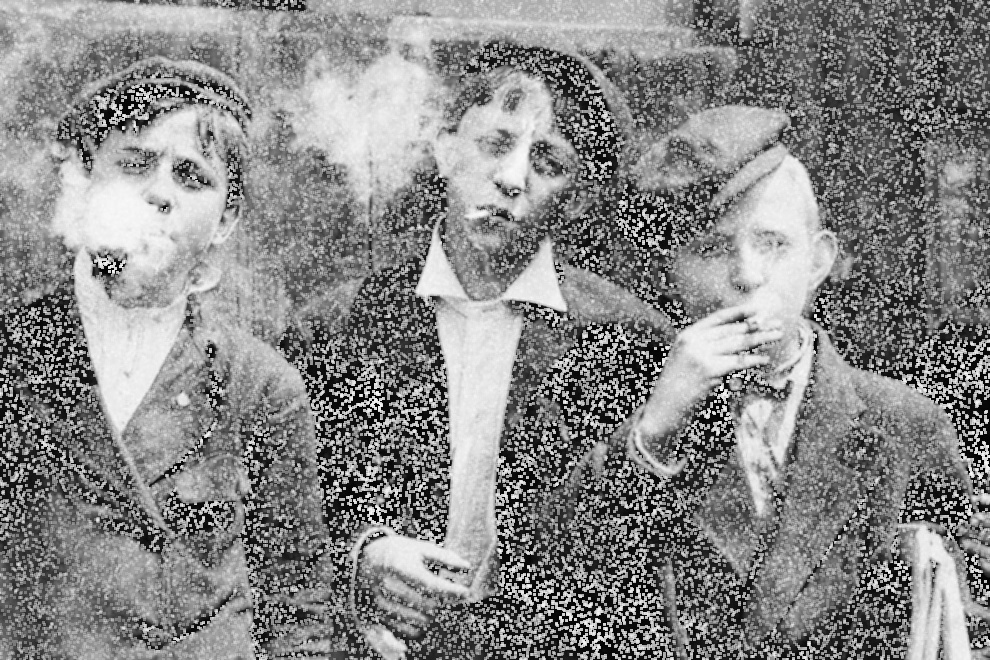
\includegraphics[width=0.95\linewidth]{../Contraharmonic_Filter/Contraharmonic_Impulse_noise_(m,n=(3,_3),q=0.85).jpg} 
      \caption{Импульсный шум} 
      \label{contraharmonic_0.85:b} 
      \vspace{4ex}
    \end{subfigure}
    \begin{subfigure}[b]{0.5\linewidth}
      \centering
      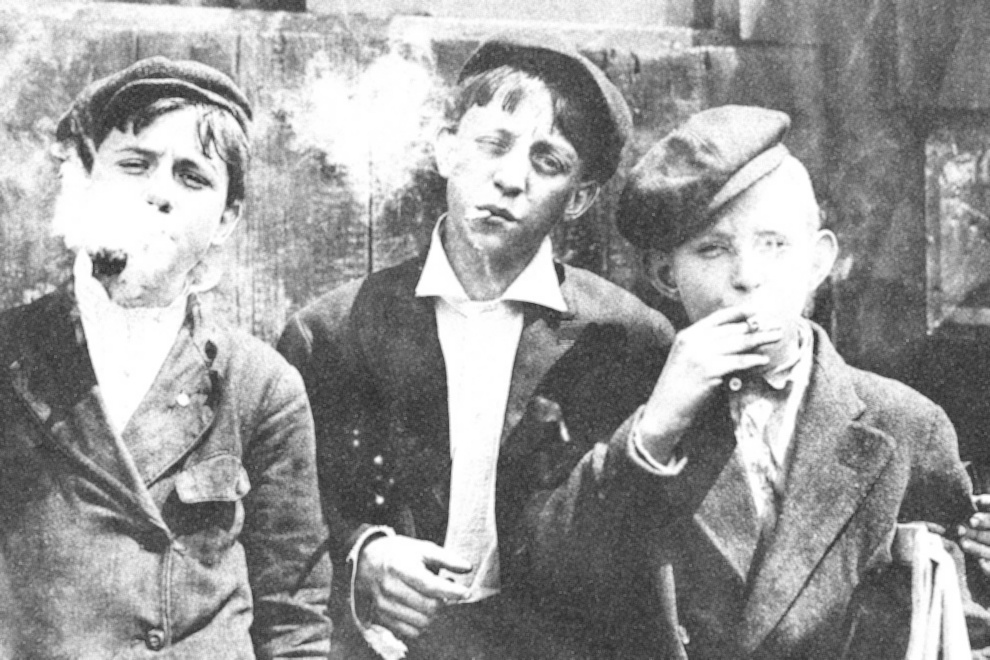
\includegraphics[width=0.95\linewidth]{../Contraharmonic_Filter/Contraharmonic_Additive_noise_(m,n=(3,_3),q=0.85).jpg} 
      \caption{Аддитивный шум} 
      \label{contraharmonic_0.85:c} 
      \vspace{4ex}
    \end{subfigure}%%
    \begin{subfigure}[b]{0.5\linewidth}
      \centering
      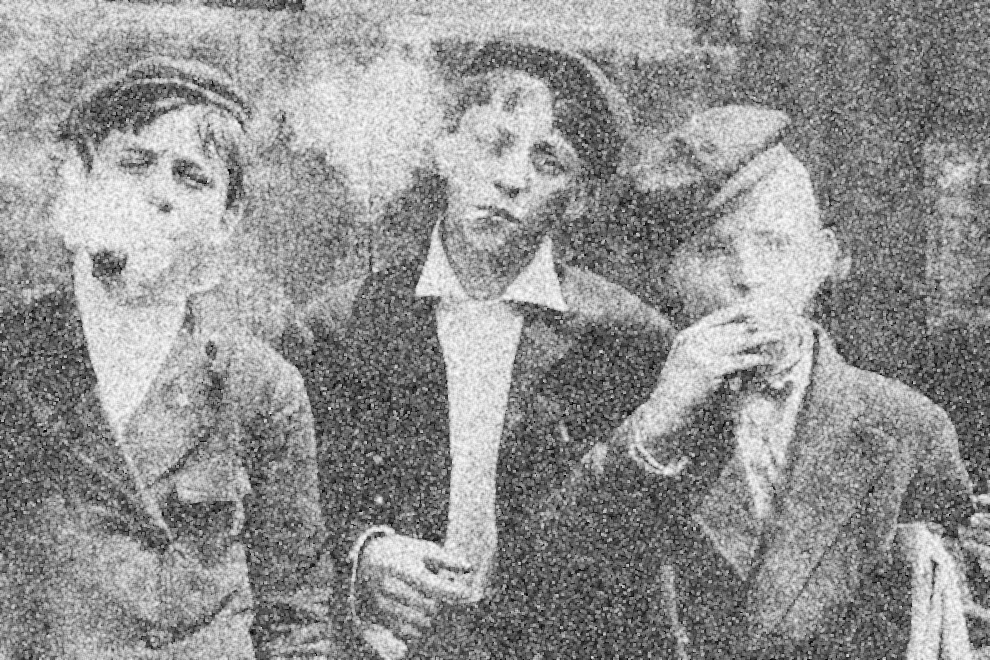
\includegraphics[width=0.95\linewidth]{../Contraharmonic_Filter/Contraharmonic_Gaussian_noise_(m,n=(3,_3),q=0.85).jpg} 
      \caption{Гауссов шум} 
      \label{contraharmonic_0.85:d} 
      \vspace{4ex}
    \end{subfigure}
    \begin{subfigure}[b]{0.5\linewidth}
      \centering
      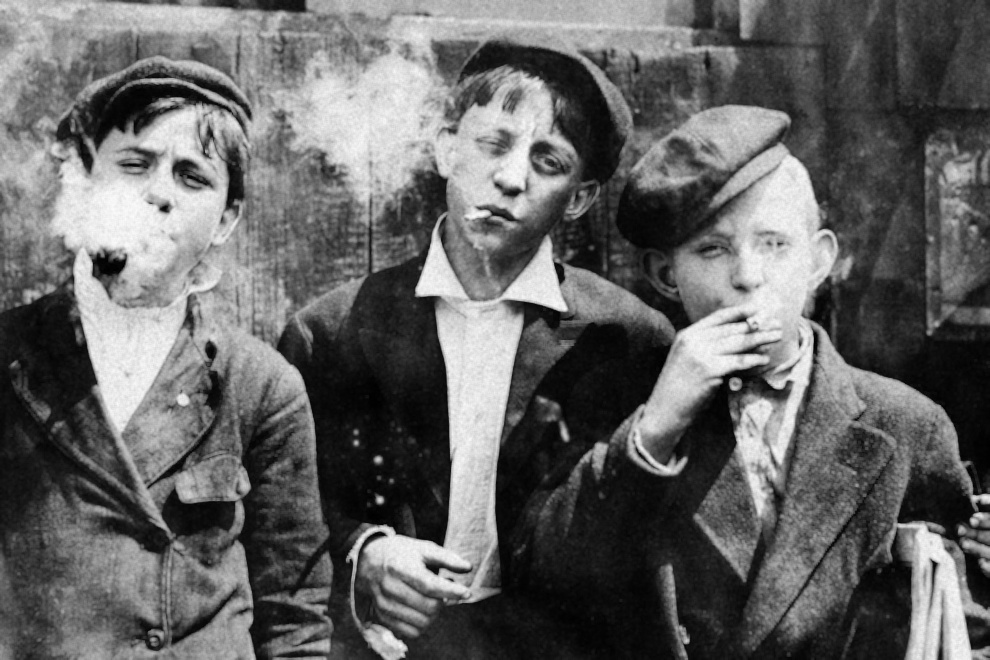
\includegraphics[width=0.95\linewidth]{../Contraharmonic_Filter/Contraharmonic_Poisson_noise_(m,n=(3,_3),q=0.85).jpg} 
      \caption{Шум квантования} 
      \label{contraharmonic_0.85:e}
    \end{subfigure}%% 
    \begin{subfigure}[b]{0.5\linewidth}
        \centering
        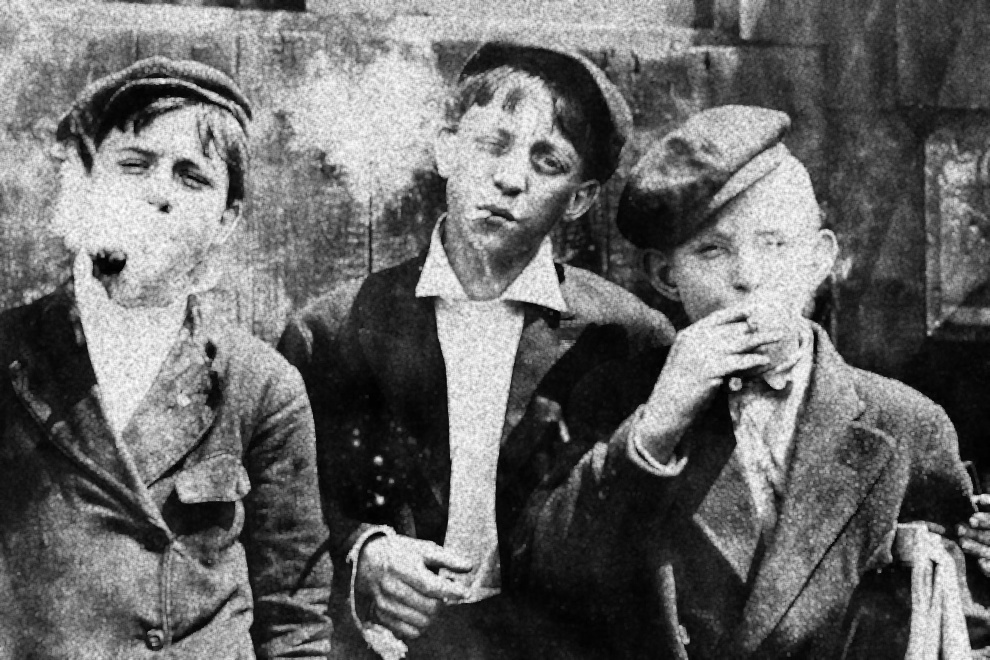
\includegraphics[width=0.95\linewidth]{../Contraharmonic_Filter/Contraharmonic_Speckle_noise_(m,n=(3,_3),q=0.85).jpg} 
        \caption{Мультипликативный шум} 
        \label{contraharmonic_0.85:f} 
    \end{subfigure} 
    \caption{Результат применения контргармонического усредняющего фильтра при значении $Q = 0.85$ к различным типам шумов}
    \label{img:contraharmonic_0.85} 
  \end{figure}

  \begin{figure}[ht!] 
    \centering
    \begin{subfigure}[b]{0.5\linewidth}
        \centering
        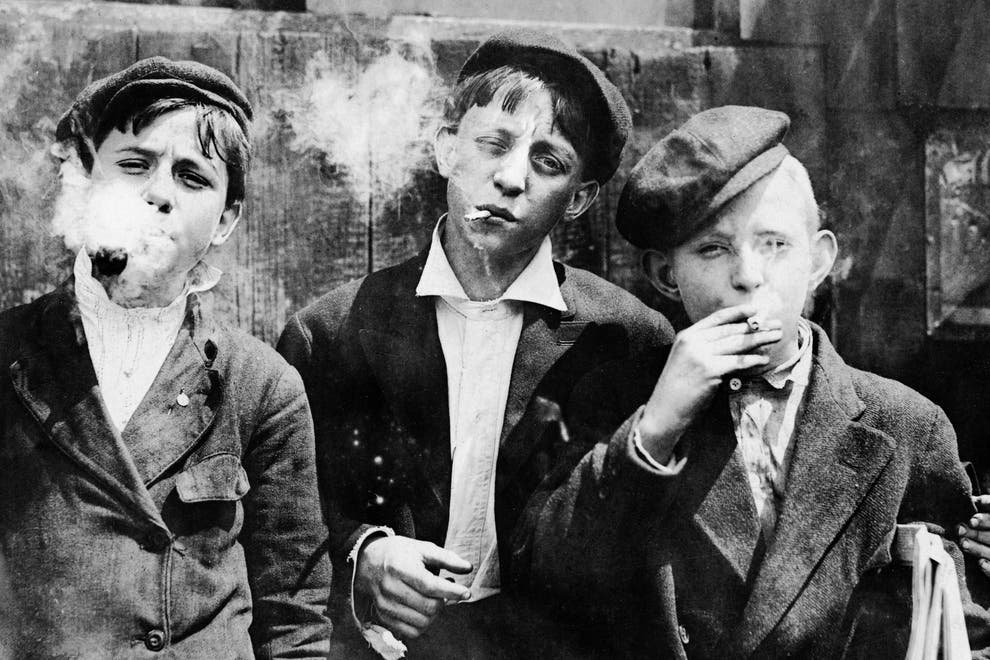
\includegraphics[width=0.95\linewidth]{../lewis-hine-taschen-main-3.jpg} 
        \caption{Исходное изображение} 
        \label{contraharmonic_1.85:a} 
        \vspace{4ex}
    \end{subfigure}%%
    \begin{subfigure}[b]{0.5\linewidth}
      \centering
      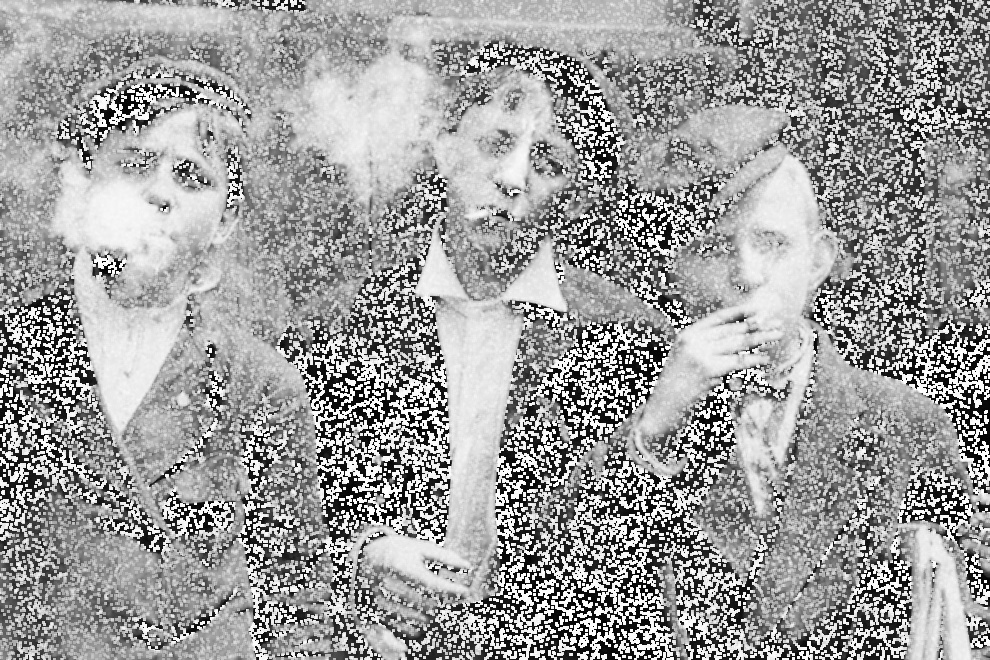
\includegraphics[width=0.95\linewidth]{../Contraharmonic_Filter/Contraharmonic_Impulse_noise_(m,n=(3,_3),q=1.85).jpg} 
      \caption{Импульсный шум} 
      \label{contraharmonic_1.85:b} 
      \vspace{4ex}
    \end{subfigure}
    \begin{subfigure}[b]{0.5\linewidth}
      \centering
      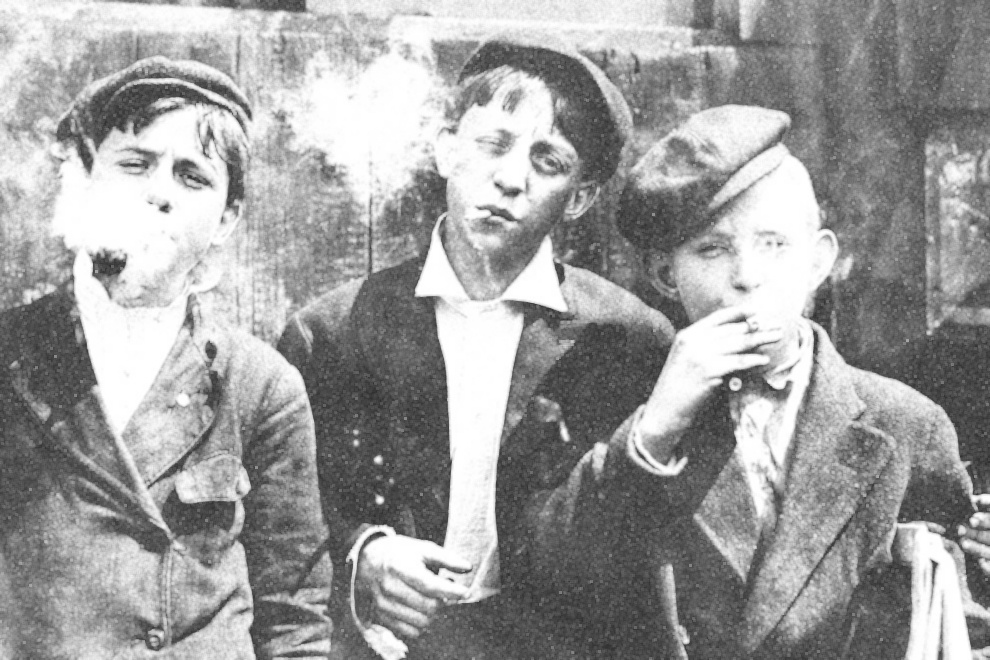
\includegraphics[width=0.95\linewidth]{../Contraharmonic_Filter/Contraharmonic_Additive_noise_(m,n=(3,_3),q=1.85).jpg} 
      \caption{Аддитивный шум} 
      \label{contraharmonic_1.85:c} 
      \vspace{4ex}
    \end{subfigure}%%
    \begin{subfigure}[b]{0.5\linewidth}
      \centering
      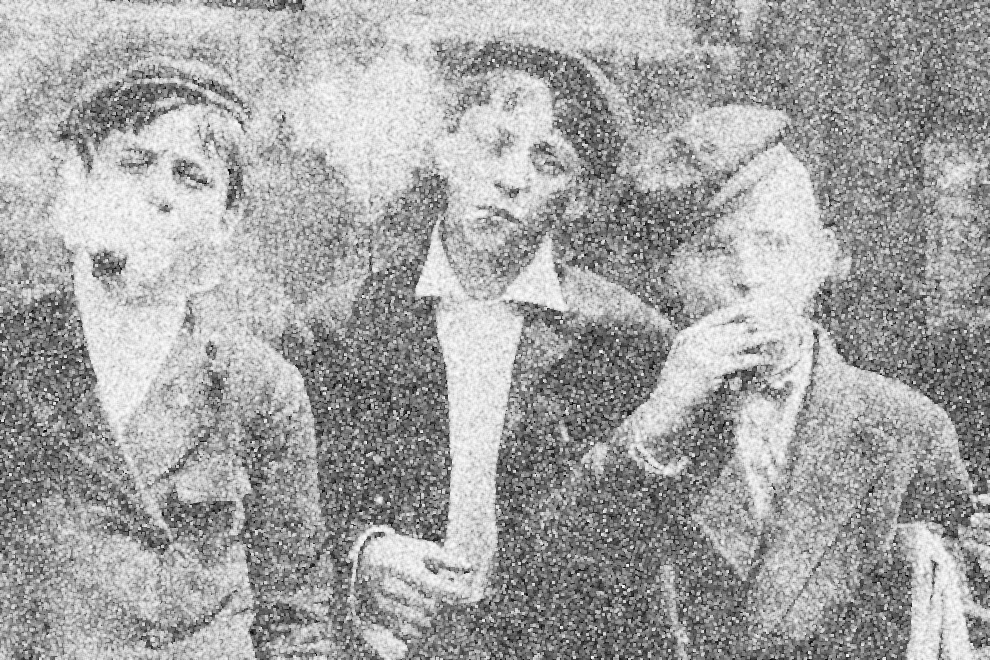
\includegraphics[width=0.95\linewidth]{../Contraharmonic_Filter/Contraharmonic_Gaussian_noise_(m,n=(3,_3),q=1.85).jpg} 
      \caption{Гауссов шум} 
      \label{contraharmonic_1.85:d} 
      \vspace{4ex}
    \end{subfigure}
    \begin{subfigure}[b]{0.5\linewidth}
      \centering
      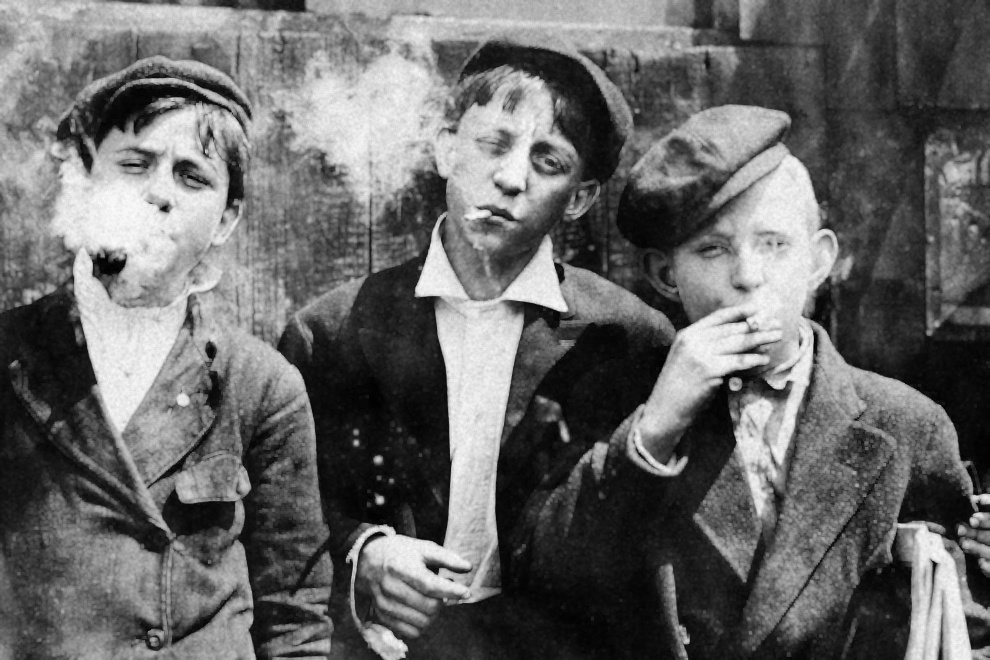
\includegraphics[width=0.95\linewidth]{../Contraharmonic_Filter/Contraharmonic_Poisson_noise_(m,n=(3,_3),q=1.85).jpg} 
      \caption{Шум квантования} 
      \label{contraharmonic_1.85:e}
    \end{subfigure}%% 
    \begin{subfigure}[b]{0.5\linewidth}
        \centering
        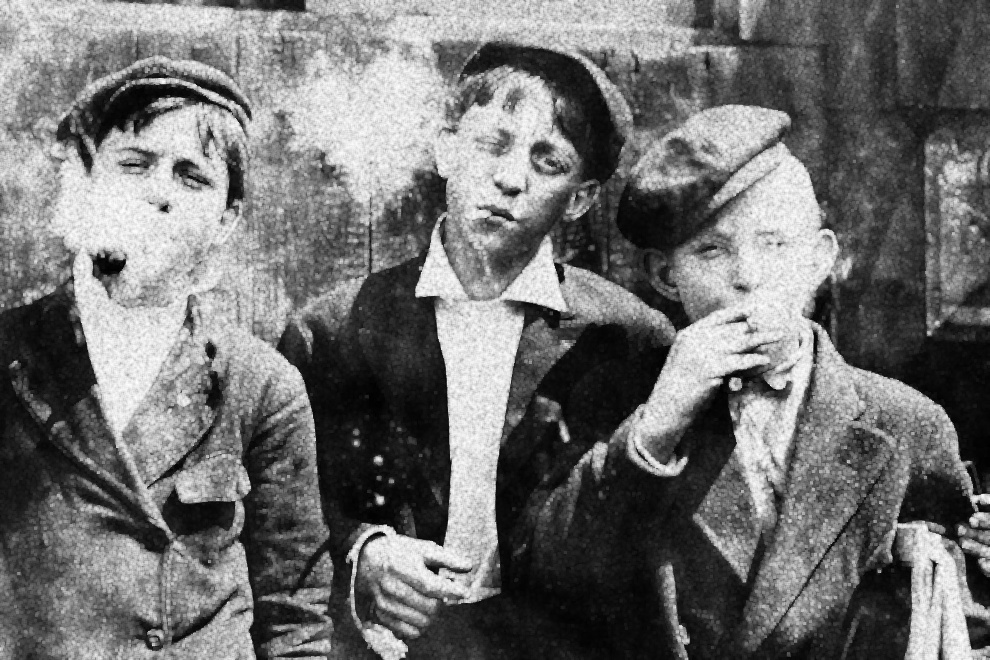
\includegraphics[width=0.95\linewidth]{../Contraharmonic_Filter/Contraharmonic_Speckle_noise_(m,n=(3,_3),q=1.85).jpg} 
        \caption{Мультипликативный шум} 
        \label{contraharmonic_1.85:f} 
    \end{subfigure} 
    \caption{Результат применения контргармонического усредняющего фильтра при значении $Q = 1.85$ к различным типам шумов}
    \label{img:contraharmonic_1.85} 
  \end{figure}

  \FloatBarrier

\subsubsection{Фильтр Гаусса}
При фильтрации изображений будем использовать двумерный фильтр Гаусса:
\begin{equation}
   G_\sigma = \frac{1}{2\pi\sigma^2} e^{-\frac{x^2+y^2}{2\sigma^2}} = \frac{1}{\sigma\sqrt{2\pi}} e^{\frac{-x^2}{2\sigma^2}} \cdot \frac{1}{\sigma\sqrt{2\pi}} e^{\frac{-y^2}{2\sigma^2}}
\end{equation}

\begin{figure}[ht!] 
    \centering
    \begin{subfigure}[b]{0.5\linewidth}
        \centering
        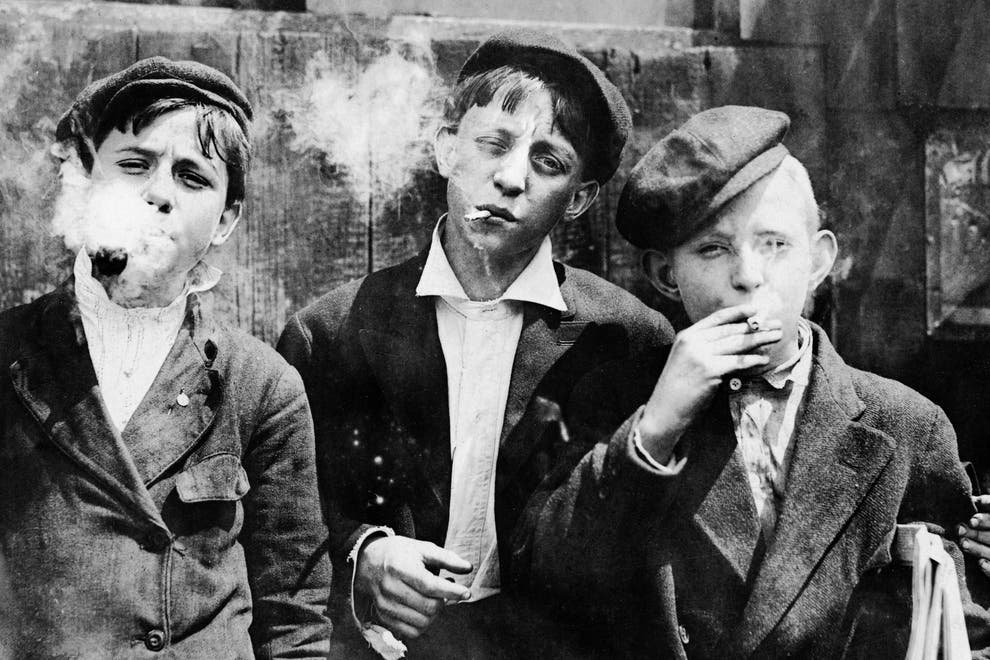
\includegraphics[width=0.95\linewidth]{../lewis-hine-taschen-main-3.jpg} 
        \caption{Исходное изображение} 
        \label{gaussian_3:a} 
        \vspace{4ex}
    \end{subfigure}%%
    \begin{subfigure}[b]{0.5\linewidth}
      \centering
      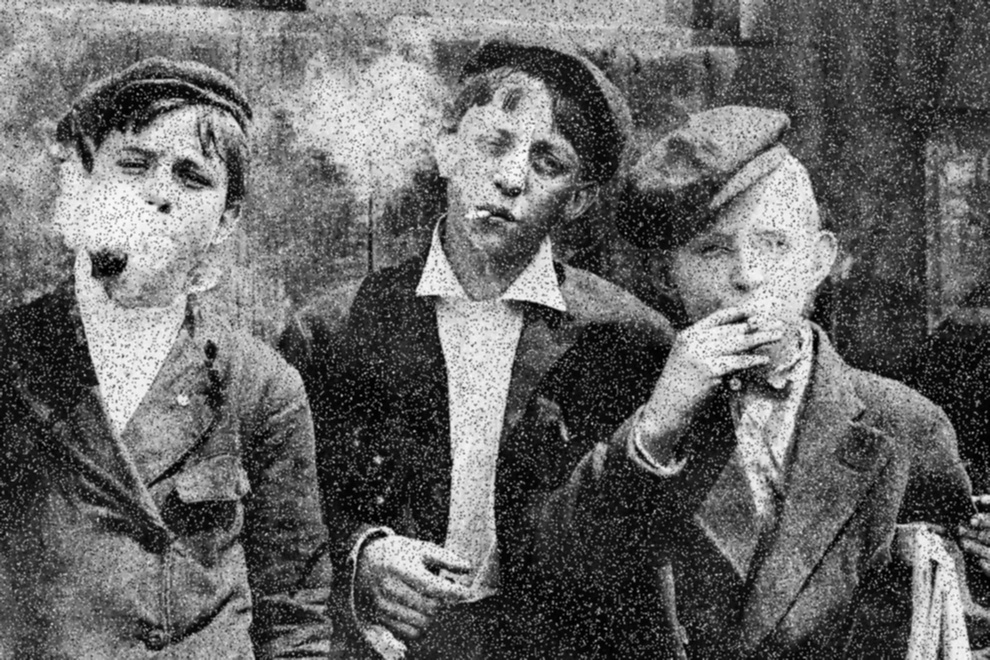
\includegraphics[width=0.95\linewidth]{../Gaussian_Blur/Gaussian_Blur_Impulse_noise_(3,3).jpg} 
      \caption{Импульсный шум} 
      \label{gaussian_3:b} 
      \vspace{4ex}
    \end{subfigure}
    \begin{subfigure}[b]{0.5\linewidth}
      \centering
      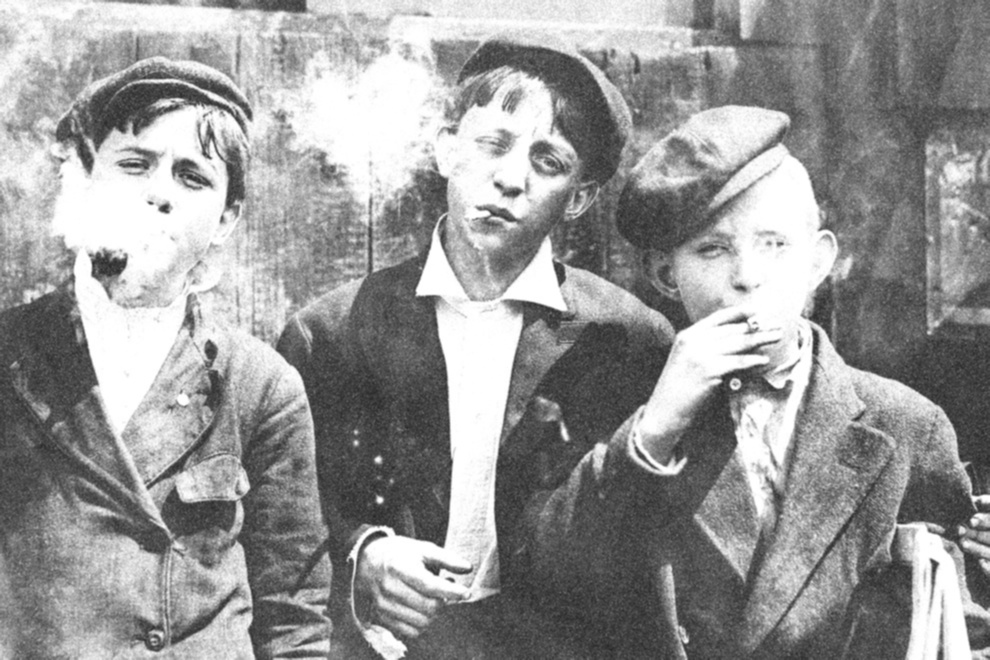
\includegraphics[width=0.95\linewidth]{../Gaussian_Blur/Gaussian_Blur_Additive_noise_(3,3).jpg} 
      \caption{Аддитивный шум} 
      \label{gaussian_3:c} 
      \vspace{4ex}
    \end{subfigure}%%
    \begin{subfigure}[b]{0.5\linewidth}
      \centering
      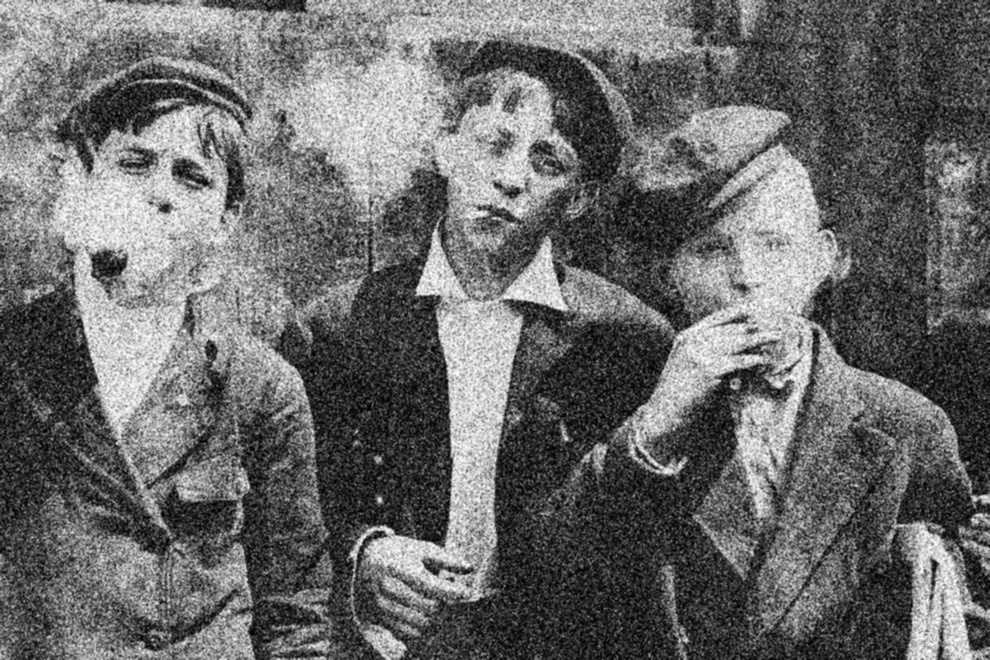
\includegraphics[width=0.95\linewidth]{../Gaussian_Blur/Gaussian_Blur_Gaussian_noise_(3,3).jpg} 
      \caption{Гауссов шум} 
      \label{gaussian_3:d} 
      \vspace{4ex}
    \end{subfigure}
    \begin{subfigure}[b]{0.5\linewidth}
      \centering
      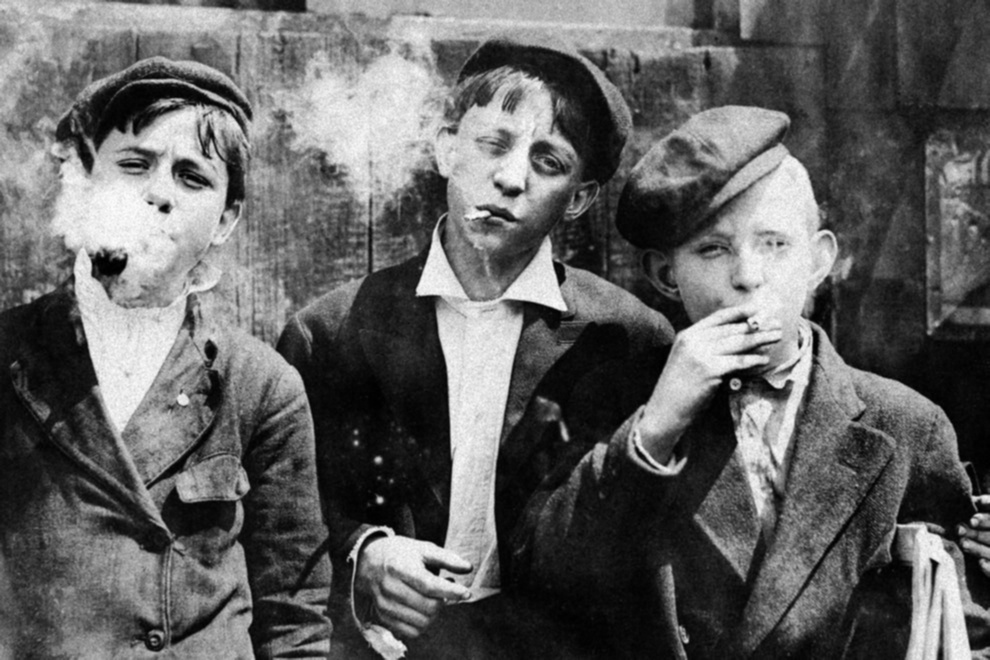
\includegraphics[width=0.95\linewidth]{../Gaussian_Blur/Gaussian_Blur_Poisson_noise_(3,3).jpg} 
      \caption{Шум квантования} 
      \label{gaussian_3:e}
    \end{subfigure}%% 
    \begin{subfigure}[b]{0.5\linewidth}
        \centering
        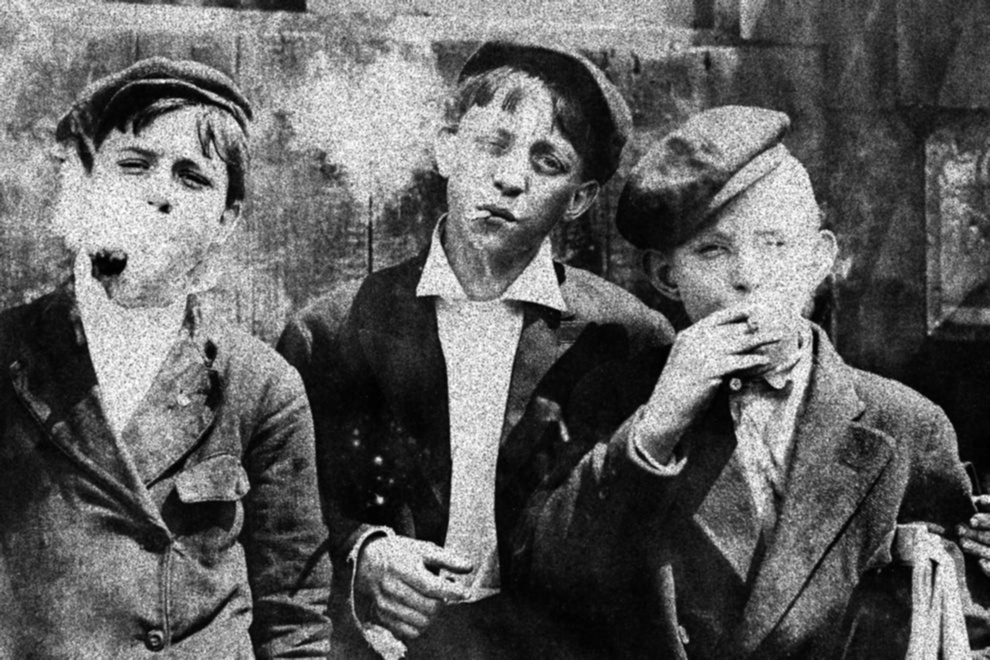
\includegraphics[width=0.95\linewidth]{../Gaussian_Blur/Gaussian_Blur_Speckle_noise_(3,3).jpg} 
        \caption{Мультипликативный шум} 
        \label{gaussian_3:f} 
    \end{subfigure} 
    \caption{Результат применения фильтра Гаусса к различным типам шумов при $n = 3$}
    \label{img:gaussian_3} 
  \end{figure}

  \begin{figure}[ht!] 
    \centering
    \begin{subfigure}[b]{0.5\linewidth}
        \centering
        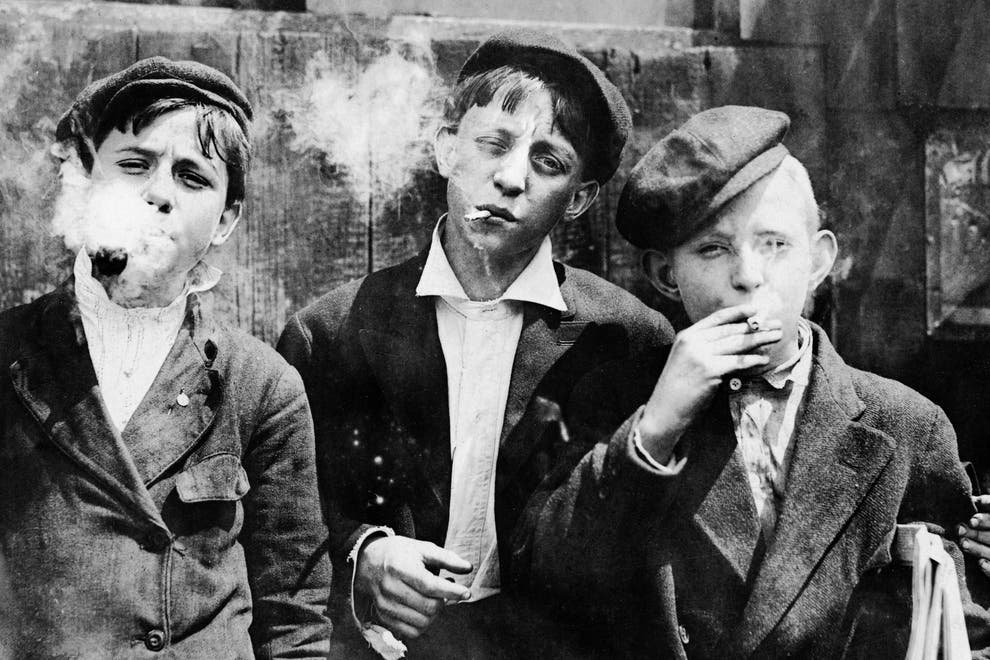
\includegraphics[width=0.95\linewidth]{../lewis-hine-taschen-main-3.jpg} 
        \caption{Исходное изображение} 
        \label{gaussian_7:a} 
        \vspace{4ex}
    \end{subfigure}%%
    \begin{subfigure}[b]{0.5\linewidth}
      \centering
      \includegraphics[width=0.95\linewidth]{../Gaussian_Blur/Gaussian_Blur_Impulse_noise_(7,7).jpg} 
      \caption{Импульсный шум} 
      \label{gaussian_7:b} 
      \vspace{4ex}
    \end{subfigure}
    \begin{subfigure}[b]{0.5\linewidth}
      \centering
      \includegraphics[width=0.95\linewidth]{../Gaussian_Blur/Gaussian_Blur_Additive_noise_(7,7).jpg} 
      \caption{Аддитивный шум} 
      \label{gaussian_7:c} 
      \vspace{4ex}
    \end{subfigure}%%
    \begin{subfigure}[b]{0.5\linewidth}
      \centering
      \includegraphics[width=0.95\linewidth]{../Gaussian_Blur/Gaussian_Blur_Gaussian_noise_(7,7).jpg} 
      \caption{Гауссов шум} 
      \label{gaussian_7:d} 
      \vspace{4ex}
    \end{subfigure}
    \begin{subfigure}[b]{0.5\linewidth}
      \centering
      \includegraphics[width=0.95\linewidth]{../Gaussian_Blur/Gaussian_Blur_Poisson_noise_(7,7).jpg} 
      \caption{Шум квантования} 
      \label{gaussian_7:e}
    \end{subfigure}%% 
    \begin{subfigure}[b]{0.5\linewidth}
        \centering
        \includegraphics[width=0.95\linewidth]{../Gaussian_Blur/Gaussian_Blur_Speckle_noise_(7,7).jpg} 
        \caption{Мультипликативный шум} 
        \label{gaussian_7:f} 
    \end{subfigure} 
    \caption{Результат применения фильтра Гаусса к различным типам шумов при $n = 7$}
    \label{img:gaussian_7} 
  \end{figure}

  \begin{figure}[ht!] 
    \centering
    \begin{subfigure}[b]{0.5\linewidth}
        \centering
        \includegraphics[width=0.95\linewidth]{../lewis-hine-taschen-main-3.jpg} 
        \caption{Исходное изображение} 
        \label{gaussian_11:a} 
        \vspace{4ex}
    \end{subfigure}%%
    \begin{subfigure}[b]{0.5\linewidth}
      \centering
      \includegraphics[width=0.95\linewidth]{../Gaussian_Blur/Gaussian_Blur_Impulse_noise_(11,11).jpg} 
      \caption{Импульсный шум} 
      \label{gaussian_11:b} 
      \vspace{4ex}
    \end{subfigure}
    \begin{subfigure}[b]{0.5\linewidth}
      \centering
      \includegraphics[width=0.95\linewidth]{../Gaussian_Blur/Gaussian_Blur_Additive_noise_(11,11).jpg} 
      \caption{Аддитивный шум} 
      \label{gaussian_11:c} 
      \vspace{4ex}
    \end{subfigure}%%
    \begin{subfigure}[b]{0.5\linewidth}
      \centering
      \includegraphics[width=0.95\linewidth]{../Gaussian_Blur/Gaussian_Blur_Gaussian_noise_(11,11).jpg} 
      \caption{Гауссов шум} 
      \label{gaussian_11:d} 
      \vspace{4ex}
    \end{subfigure}
    \begin{subfigure}[b]{0.5\linewidth}
      \centering
      \includegraphics[width=0.95\linewidth]{../Gaussian_Blur/Gaussian_Blur_Poisson_noise_(11,11).jpg} 
      \caption{Шум квантования} 
      \label{gaussian_11:e}
    \end{subfigure}%% 
    \begin{subfigure}[b]{0.5\linewidth}
        \centering
        \includegraphics[width=0.95\linewidth]{../Gaussian_Blur/Gaussian_Blur_Speckle_noise_(11,11).jpg} 
        \caption{Мультипликативный шум} 
        \label{gaussian_11:f} 
    \end{subfigure} 
    \caption{Результат применения фильтра Гаусса к различным типам шумов при $n = 11$}
    \label{img:gaussian_11} 
\end{figure}
  \FloatBarrier

\subsection{Нелинейная фильтрация}

\subsubsection{Медианная фильтрация}

\begin{figure}[ht!] 
    \centering
    \begin{subfigure}[b]{0.5\linewidth}
        \centering
        \includegraphics[width=0.95\linewidth]{../lewis-hine-taschen-main-3.jpg} 
        \caption{Исходное изображение} 
        \label{median_3:a} 
        \vspace{4ex}
    \end{subfigure}%%
    \begin{subfigure}[b]{0.5\linewidth}
      \centering
      \includegraphics[width=0.95\linewidth]{../Median_FIlter/Median_Impulse_noise_(k=3).jpg} 
      \caption{Импульсный шум} 
      \label{median_3:b} 
      \vspace{4ex}
    \end{subfigure}
    \begin{subfigure}[b]{0.5\linewidth}
      \centering
      \includegraphics[width=0.95\linewidth]{../Median_FIlter/Median_Additive_noise_(k=3).jpg} 
      \caption{Аддитивный шум} 
      \label{median_3:c} 
      \vspace{4ex}
    \end{subfigure}%%
    \begin{subfigure}[b]{0.5\linewidth}
      \centering
      \includegraphics[width=0.95\linewidth]{../Median_FIlter/Median_Gaussian_noise_(k=3).jpg} 
      \caption{Гауссов шум} 
      \label{median_3:d} 
      \vspace{4ex}
    \end{subfigure}
    \begin{subfigure}[b]{0.5\linewidth}
      \centering
      \includegraphics[width=0.95\linewidth]{../Median_FIlter/Median_Poisson_noise_(k=3).jpg} 
      \caption{Шум квантования} 
      \label{median_3:e}
    \end{subfigure}%% 
    \begin{subfigure}[b]{0.5\linewidth}
        \centering
        \includegraphics[width=0.95\linewidth]{../Median_FIlter/Median_Speckle_noise_(k=3).jpg} 
        \caption{Мультипликативный шум} 
        \label{median_3:f} 
    \end{subfigure} 
    \caption{Результат применения медианной фильтрации к различным типам шумов при $k = 3$}
    \label{img:median_3} 
\end{figure}

\begin{figure}[ht!] 
    \centering
    \begin{subfigure}[b]{0.5\linewidth}
        \centering
        \includegraphics[width=0.95\linewidth]{../lewis-hine-taschen-main-3.jpg} 
        \caption{Исходное изображение} 
        \label{median_5:a} 
        \vspace{4ex}
    \end{subfigure}%%
    \begin{subfigure}[b]{0.5\linewidth}
      \centering
      \includegraphics[width=0.95\linewidth]{../Median_FIlter/Median_Impulse_noise_(k=5).jpg} 
      \caption{Импульсный шум} 
      \label{median_5:b} 
      \vspace{4ex}
    \end{subfigure}
    \begin{subfigure}[b]{0.5\linewidth}
      \centering
      \includegraphics[width=0.95\linewidth]{../Median_FIlter/Median_Additive_noise_(k=5).jpg} 
      \caption{Аддитивный шум} 
      \label{median_5:c} 
      \vspace{4ex}
    \end{subfigure}%%
    \begin{subfigure}[b]{0.5\linewidth}
      \centering
      \includegraphics[width=0.95\linewidth]{../Median_FIlter/Median_Gaussian_noise_(k=5).jpg} 
      \caption{Гауссов шум} 
      \label{median_5:d} 
      \vspace{4ex}
    \end{subfigure}
    \begin{subfigure}[b]{0.5\linewidth}
      \centering
      \includegraphics[width=0.95\linewidth]{../Median_FIlter/Median_Poisson_noise_(k=5).jpg} 
      \caption{Шум квантования} 
      \label{median_5:e}
    \end{subfigure}%% 
    \begin{subfigure}[b]{0.5\linewidth}
        \centering
        \includegraphics[width=0.95\linewidth]{../Median_FIlter/Median_Speckle_noise_(k=5).jpg} 
        \caption{Мультипликативный шум} 
        \label{median_5:f} 
    \end{subfigure} 
    \caption{Результат применения медианной фильтрации к различным типам шумов при $k = 5$}
    \label{img:median_5} 
\end{figure}

\begin{figure}[ht!] 
    \centering
    \begin{subfigure}[b]{0.5\linewidth}
        \centering
        \includegraphics[width=0.95\linewidth]{../lewis-hine-taschen-main-3.jpg} 
        \caption{Исходное изображение} 
        \label{median_7:a} 
        \vspace{4ex}
    \end{subfigure}%%
    \begin{subfigure}[b]{0.5\linewidth}
      \centering
      \includegraphics[width=0.95\linewidth]{../Median_FIlter/Median_Impulse_noise_(k=7).jpg} 
      \caption{Импульсный шум} 
      \label{median_7:b} 
      \vspace{4ex}
    \end{subfigure}
    \begin{subfigure}[b]{0.5\linewidth}
      \centering
      \includegraphics[width=0.95\linewidth]{../Median_FIlter/Median_Additive_noise_(k=7).jpg} 
      \caption{Аддитивный шум} 
      \label{median_7:c} 
      \vspace{4ex}
    \end{subfigure}%%
    \begin{subfigure}[b]{0.5\linewidth}
      \centering
      \includegraphics[width=0.95\linewidth]{../Median_FIlter/Median_Gaussian_noise_(k=7).jpg} 
      \caption{Гауссов шум} 
      \label{median_7:d} 
      \vspace{4ex}
    \end{subfigure}
    \begin{subfigure}[b]{0.5\linewidth}
      \centering
      \includegraphics[width=0.95\linewidth]{../Median_FIlter/Median_Poisson_noise_(k=7).jpg} 
      \caption{Шум квантования} 
      \label{median_7:e}
    \end{subfigure}%% 
    \begin{subfigure}[b]{0.5\linewidth}
        \centering
        \includegraphics[width=0.95\linewidth]{../Median_FIlter/Median_Speckle_noise_(k=7).jpg} 
        \caption{Мультипликативный шум} 
        \label{median_7:f} 
    \end{subfigure} 
    \caption{Результат применения медианной фильтрации к различным типам шумов при $k = 7$}
    \label{img:median_7} 
\end{figure}
\FloatBarrier

\subsubsection{Взвешенная медианная фильтрация}


\begin{figure}[ht!] 
    \centering
    \begin{subfigure}[b]{0.5\linewidth}
        \centering
        \includegraphics[width=0.95\linewidth]{../lewis-hine-taschen-main-3.jpg} 
        \caption{Исходное изображение} 
        \label{median2d_3:a} 
        \vspace{4ex}
    \end{subfigure}%%
    \begin{subfigure}[b]{0.5\linewidth}
      \centering
      \includegraphics[width=0.95\linewidth]{../Median_2D_Filter/Median_2DImpulse_noise_(k=3).jpg} 
      \caption{Импульсный шум} 
      \label{median2d_3:b} 
      \vspace{4ex}
    \end{subfigure}
    \begin{subfigure}[b]{0.5\linewidth}
      \centering
      \includegraphics[width=0.95\linewidth]{../Median_2D_Filter/Median_2DAdditive_noise_(k=3).jpg} 
      \caption{Аддитивный шум} 
      \label{median2d_3:c} 
      \vspace{4ex}
    \end{subfigure}%%
    \begin{subfigure}[b]{0.5\linewidth}
      \centering
      \includegraphics[width=0.95\linewidth]{../Median_2D_Filter/Median_2DGaussian_noise_(k=3).jpg} 
      \caption{Гауссов шум} 
      \label{median2d_3:d} 
      \vspace{4ex}
    \end{subfigure}
    \begin{subfigure}[b]{0.5\linewidth}
      \centering
      \includegraphics[width=0.95\linewidth]{../Median_2D_Filter/Median_2DPoisson_noise_(k=3).jpg} 
      \caption{Шум квантования} 
      \label{median2d_3:e}
    \end{subfigure}%% 
    \begin{subfigure}[b]{0.5\linewidth}
        \centering
        \includegraphics[width=0.95\linewidth]{../Median_2D_Filter/Median_2DSpeckle_noise_(k=3).jpg} 
        \caption{Мультипликативный шум} 
        \label{median2d_3:f} 
    \end{subfigure} 
    \caption{Результат применения взвешенной медианной фильтрации к различным типам шумов при $k = 3$}
    \label{img:median2d_3} 
\end{figure}

\begin{figure}[ht!] 
    \centering
    \begin{subfigure}[b]{0.5\linewidth}
        \centering
        \includegraphics[width=0.95\linewidth]{../lewis-hine-taschen-main-3.jpg} 
        \caption{Исходное изображение} 
        \label{median2d_5:a} 
        \vspace{4ex}
    \end{subfigure}%%
    \begin{subfigure}[b]{0.5\linewidth}
      \centering
      \includegraphics[width=0.95\linewidth]{../Median_2D_Filter/Median_2DImpulse_noise_(k=5).jpg} 
      \caption{Импульсный шум} 
      \label{median2d_5:b} 
      \vspace{4ex}
    \end{subfigure}
    \begin{subfigure}[b]{0.5\linewidth}
      \centering
      \includegraphics[width=0.95\linewidth]{../Median_2D_Filter/Median_2DAdditive_noise_(k=5).jpg} 
      \caption{Аддитивный шум} 
      \label{median2d_5:c} 
      \vspace{4ex}
    \end{subfigure}%%
    \begin{subfigure}[b]{0.5\linewidth}
      \centering
      \includegraphics[width=0.95\linewidth]{../Median_2D_Filter/Median_2DGaussian_noise_(k=5).jpg} 
      \caption{Гауссов шум} 
      \label{median2d_5:d} 
      \vspace{4ex}
    \end{subfigure}
    \begin{subfigure}[b]{0.5\linewidth}
      \centering
      \includegraphics[width=0.95\linewidth]{../Median_2D_Filter/Median_2DPoisson_noise_(k=5).jpg} 
      \caption{Шум квантования} 
      \label{median2d_5:e}
    \end{subfigure}%% 
    \begin{subfigure}[b]{0.5\linewidth}
        \centering
        \includegraphics[width=0.95\linewidth]{../Median_2D_Filter/Median_2DSpeckle_noise_(k=5).jpg} 
        \caption{Мультипликативный шум} 
        \label{median2d_5:f} 
    \end{subfigure} 
    \caption{Результат применения взвешенной медианной фильтрации к различным типам шумов при $k = 5$}
    \label{img:median2d_5} 
\end{figure}

\begin{figure}[ht!] 
    \centering
    \begin{subfigure}[b]{0.5\linewidth}
        \centering
        \includegraphics[width=0.95\linewidth]{../lewis-hine-taschen-main-3.jpg} 
        \caption{Исходное изображение} 
        \label{median2d_7:a} 
        \vspace{4ex}
    \end{subfigure}%%
    \begin{subfigure}[b]{0.5\linewidth}
      \centering
      \includegraphics[width=0.95\linewidth]{../Median_2D_Filter/Median_2DImpulse_noise_(k=7).jpg} 
      \caption{Импульсный шум} 
      \label{median2d_7:b} 
      \vspace{4ex}
    \end{subfigure}
    \begin{subfigure}[b]{0.5\linewidth}
      \centering
      \includegraphics[width=0.95\linewidth]{../Median_2D_Filter/Median_2DAdditive_noise_(k=7).jpg} 
      \caption{Аддитивный шум} 
      \label{median2d_7:c} 
      \vspace{4ex}
    \end{subfigure}%%
    \begin{subfigure}[b]{0.5\linewidth}
      \centering
      \includegraphics[width=0.95\linewidth]{../Median_2D_Filter/Median_2DGaussian_noise_(k=7).jpg} 
      \caption{Гауссов шум} 
      \label{median2d_7:d} 
      \vspace{4ex}
    \end{subfigure}
    \begin{subfigure}[b]{0.5\linewidth}
      \centering
      \includegraphics[width=0.95\linewidth]{../Median_2D_Filter/Median_2DPoisson_noise_(k=7).jpg} 
      \caption{Шум квантования} 
      \label{median2d_7:e}
    \end{subfigure}%% 
    \begin{subfigure}[b]{0.5\linewidth}
        \centering
        \includegraphics[width=0.95\linewidth]{../Median_2D_Filter/Median_2DSpeckle_noise_(k=7).jpg} 
        \caption{Мультипликативный шум} 
        \label{median2d_7:f} 
    \end{subfigure} 
    \caption{Результат применения взвешенной медианной фильтрации к различным типам шумов при $k = 7$}
    \label{img:median2d_7} 
\end{figure}
\FloatBarrier


\subsubsection{Адаптивная медианная фильтрация}

Обозначим через $z_{min},~z_{max},~z_{med}$ минимальное, максимальное и медианное значения интенсивностей в окне, $z_{i,j}$ — значение интенсивности пикселя с координатами $(i, j), s_{max}$ — максимально допустимый размер окна.
Алгоритм адаптивной медианной фильтрации
состоит из следующих шагов: \\
\begin{enumerate}
    \item Вычисление значений $z_{min}, z_{max}, z_{med}, A_1 =  z_{med} - z_{min}, A_2 = z_{med} - z_{max}$ пикселя $(i, j)$ в заданном окне. \\
    (a) Если $A_1 > 0 $ и $A_2 < 0$, перейти на шаг 2. В противном случае увеличить размер окна. \\
    (b) Если текущий размер окна $s \le s_{max}$, повторить шаг 1. В
противном случае результат фильтрации равен $z_{i,j}$. 
    \item Вычисление значений $B_1 = z_{i,j} - z_{min}, B_2 = z_{i,j} - z_{max}$. \\
    (a) Если $B_1 > 0$ и $B_2 < 0$, результат фильтрации равен $z_{i,j}$.
    В противном случае результат фильтрации равен $z_{med}$.

    \item Изменение координат $(i,j)$.
    (a) Если не достигнут предел изображения, перейти на шаг 1. В противном случае фильтрация окончена.
\end{enumerate}


Основной идеей является увеличение размера окна до тех пор,
пока алгоритм не найдет медианное значение, не являющееся импульсным шумом, или пока не достигнет максимального размера
окна. В последнем случае алгоритм вернет величину $z_{i,j}$.
\subsubsection{Ранговая фильтрация}

\begin{figure}[ht!] 
    \centering
    \begin{subfigure}[b]{0.5\linewidth}
        \centering
        \includegraphics[width=0.95\linewidth]{../lewis-hine-taschen-main-3.jpg} 
        \caption{Исходное изображение} 
        \label{rang_3_1:a} 
        \vspace{4ex}
    \end{subfigure}%%
    \begin{subfigure}[b]{0.5\linewidth}
      \centering
      \includegraphics[width=0.95\linewidth]{../Rang_Filter/Rang_Impulse_noise_(k=3,r=1).jpg} 
      \caption{Импульсный шум} 
      \label{rang_3_1:b} 
      \vspace{4ex}
    \end{subfigure}
    \begin{subfigure}[b]{0.5\linewidth}
      \centering
      \includegraphics[width=0.95\linewidth]{../Rang_Filter/Rang_Additive_noise_(k=3,r=1).jpg} 
      \caption{Аддитивный шум} 
      \label{rang_3_1:c} 
      \vspace{4ex}
    \end{subfigure}%%
    \begin{subfigure}[b]{0.5\linewidth}
      \centering
      \includegraphics[width=0.95\linewidth]{../Rang_Filter/Rang_Gaussian_noise_(k=3,r=1).jpg} 
      \caption{Гауссов шум} 
      \label{rang_3_1:d} 
      \vspace{4ex}
    \end{subfigure}
    \begin{subfigure}[b]{0.5\linewidth}
      \centering
      \includegraphics[width=0.95\linewidth]{../Rang_Filter/Rang_Poisson_noise_(k=3,r=1).jpg} 
      \caption{Шум квантования} 
      \label{rang_3_1:e}
    \end{subfigure}%% 
    \begin{subfigure}[b]{0.5\linewidth}
        \centering
        \includegraphics[width=0.95\linewidth]{../Rang_Filter/Rang_Speckle_noise_(k=3,r=1).jpg} 
        \caption{Мультипликативный шум} 
        \label{rang_3_1:f} 
    \end{subfigure} 
    \caption{Результат применения ранговой фильтрации к различным типам шумов при $k = 3, r = 1$}
    \label{img:rang_3_1} 
\end{figure}

\begin{figure}[ht!] 
    \centering
    \begin{subfigure}[b]{0.5\linewidth}
        \centering
        \includegraphics[width=0.95\linewidth]{../lewis-hine-taschen-main-3.jpg} 
        \caption{Исходное изображение} 
        \label{rang_3_5:a} 
        \vspace{4ex}
    \end{subfigure}%%
    \begin{subfigure}[b]{0.5\linewidth}
      \centering
      \includegraphics[width=0.95\linewidth]{../Rang_Filter/Rang_Impulse_noise_(k=3,r=5).jpg} 
      \caption{Импульсный шум} 
      \label{rang_3_5:b} 
      \vspace{4ex}
    \end{subfigure}
    \begin{subfigure}[b]{0.5\linewidth}
      \centering
      \includegraphics[width=0.95\linewidth]{../Rang_Filter/Rang_Additive_noise_(k=3,r=5).jpg} 
      \caption{Аддитивный шум} 
      \label{rang_3_5:c} 
      \vspace{4ex}
    \end{subfigure}%%
    \begin{subfigure}[b]{0.5\linewidth}
      \centering
      \includegraphics[width=0.95\linewidth]{../Rang_Filter/Rang_Gaussian_noise_(k=3,r=5).jpg} 
      \caption{Гауссов шум} 
      \label{rang_3_5:d} 
      \vspace{4ex}
    \end{subfigure}
    \begin{subfigure}[b]{0.5\linewidth}
      \centering
      \includegraphics[width=0.95\linewidth]{../Rang_Filter/Rang_Poisson_noise_(k=3,r=5).jpg} 
      \caption{Шум квантования} 
      \label{rang_3_5:e}
    \end{subfigure}%% 
    \begin{subfigure}[b]{0.5\linewidth}
        \centering
        \includegraphics[width=0.95\linewidth]{../Rang_Filter/Rang_Speckle_noise_(k=3,r=5).jpg} 
        \caption{Мультипликативный шум} 
        \label{rang_3_5:f} 
    \end{subfigure} 
    \caption{Результат применения ранговой фильтрации к различным типам шумов при $k = 3, r = 5$}
    \label{img:rang_3_5} 
\end{figure}

\begin{figure}[ht!] 
    \centering
    \begin{subfigure}[b]{0.5\linewidth}
        \centering
        \includegraphics[width=0.95\linewidth]{../lewis-hine-taschen-main-3.jpg} 
        \caption{Исходное изображение} 
        \label{rang_3_9:a} 
        \vspace{4ex}
    \end{subfigure}%%
    \begin{subfigure}[b]{0.5\linewidth}
      \centering
      \includegraphics[width=0.95\linewidth]{../Rang_Filter/Rang_Impulse_noise_(k=3,r=9).jpg} 
      \caption{Импульсный шум} 
      \label{rang_3_9:b} 
      \vspace{4ex}
    \end{subfigure}
    \begin{subfigure}[b]{0.5\linewidth}
      \centering
      \includegraphics[width=0.95\linewidth]{../Rang_Filter/Rang_Additive_noise_(k=3,r=9).jpg} 
      \caption{Аддитивный шум} 
      \label{rang_3_9:c} 
      \vspace{4ex}
    \end{subfigure}%%
    \begin{subfigure}[b]{0.5\linewidth}
      \centering
      \includegraphics[width=0.95\linewidth]{../Rang_Filter/Rang_Gaussian_noise_(k=3,r=9).jpg} 
      \caption{Гауссов шум} 
      \label{rang_3_9:d} 
      \vspace{4ex}
    \end{subfigure}
    \begin{subfigure}[b]{0.5\linewidth}
      \centering
      \includegraphics[width=0.95\linewidth]{../Rang_Filter/Rang_Poisson_noise_(k=3,r=9).jpg} 
      \caption{Шум квантования} 
      \label{rang_3_9:e}
    \end{subfigure}%% 
    \begin{subfigure}[b]{0.5\linewidth}
        \centering
        \includegraphics[width=0.95\linewidth]{../Rang_Filter/Rang_Speckle_noise_(k=3,r=9).jpg} 
        \caption{Мультипликативный шум} 
        \label{rang_3_9:f} 
    \end{subfigure} 
    \caption{Результат применения ранговой фильтрации к различным типам шумов при $k = 3, r = 9$}
    \label{img:rang_3_9} 
\end{figure}




\begin{figure}[ht!] 
    \centering
    \begin{subfigure}[b]{0.5\linewidth}
        \centering
        \includegraphics[width=0.95\linewidth]{../lewis-hine-taschen-main-3.jpg} 
        \caption{Исходное изображение} 
        \label{rang_5_1:a} 
        \vspace{4ex}
    \end{subfigure}%%
    \begin{subfigure}[b]{0.5\linewidth}
      \centering
      \includegraphics[width=0.95\linewidth]{../Rang_Filter/Rang_Impulse_noise_(k=5,r=1).jpg} 
      \caption{Импульсный шум} 
      \label{rang_5_1:b} 
      \vspace{4ex}
    \end{subfigure}
    \begin{subfigure}[b]{0.5\linewidth}
      \centering
      \includegraphics[width=0.95\linewidth]{../Rang_Filter/Rang_Additive_noise_(k=5,r=1).jpg} 
      \caption{Аддитивный шум} 
      \label{rang_5_1:c} 
      \vspace{4ex}
    \end{subfigure}%%
    \begin{subfigure}[b]{0.5\linewidth}
      \centering
      \includegraphics[width=0.95\linewidth]{../Rang_Filter/Rang_Gaussian_noise_(k=5,r=1).jpg} 
      \caption{Гауссов шум} 
      \label{rang_5_1:d} 
      \vspace{4ex}
    \end{subfigure}
    \begin{subfigure}[b]{0.5\linewidth}
      \centering
      \includegraphics[width=0.95\linewidth]{../Rang_Filter/Rang_Poisson_noise_(k=5,r=1).jpg} 
      \caption{Шум квантования} 
      \label{rang_5_1:e}
    \end{subfigure}%% 
    \begin{subfigure}[b]{0.5\linewidth}
        \centering
        \includegraphics[width=0.95\linewidth]{../Rang_Filter/Rang_Speckle_noise_(k=5,r=1).jpg} 
        \caption{Мультипликативный шум} 
        \label{rang_5_1:f} 
    \end{subfigure} 
    \caption{Результат применения ранговой фильтрации к различным типам шумов при $k = 5, r = 1$}
    \label{img:rang_5_1} 
\end{figure}

\begin{figure}[ht!] 
    \centering
    \begin{subfigure}[b]{0.5\linewidth}
        \centering
        \includegraphics[width=0.95\linewidth]{../lewis-hine-taschen-main-3.jpg} 
        \caption{Исходное изображение} 
        \label{rang_5_14:a} 
        \vspace{4ex}
    \end{subfigure}%%
    \begin{subfigure}[b]{0.5\linewidth}
      \centering
      \includegraphics[width=0.95\linewidth]{../Rang_Filter/Rang_Impulse_noise_(k=5,r=14).jpg} 
      \caption{Импульсный шум} 
      \label{rang_5_14:b} 
      \vspace{4ex}
    \end{subfigure}
    \begin{subfigure}[b]{0.5\linewidth}
      \centering
      \includegraphics[width=0.95\linewidth]{../Rang_Filter/Rang_Additive_noise_(k=5,r=14).jpg} 
      \caption{Аддитивный шум} 
      \label{rang_5_14:c} 
      \vspace{4ex}
    \end{subfigure}%%
    \begin{subfigure}[b]{0.5\linewidth}
      \centering
      \includegraphics[width=0.95\linewidth]{../Rang_Filter/Rang_Gaussian_noise_(k=5,r=14).jpg} 
      \caption{Гауссов шум} 
      \label{rang_5_14:d} 
      \vspace{4ex}
    \end{subfigure}
    \begin{subfigure}[b]{0.5\linewidth}
      \centering
      \includegraphics[width=0.95\linewidth]{../Rang_Filter/Rang_Poisson_noise_(k=5,r=14).jpg} 
      \caption{Шум квантования} 
      \label{rang_5_14:e}
    \end{subfigure}%% 
    \begin{subfigure}[b]{0.5\linewidth}
        \centering
        \includegraphics[width=0.95\linewidth]{../Rang_Filter/Rang_Speckle_noise_(k=5,r=14).jpg} 
        \caption{Мультипликативный шум} 
        \label{rang_5_14:f} 
    \end{subfigure} 
    \caption{Результат применения ранговой фильтрации к различным типам шумов при $k = 5, r = 14$}
    \label{img:rang_5_14} 
\end{figure}

\begin{figure}[ht!] 
    \centering
    \begin{subfigure}[b]{0.5\linewidth}
        \centering
        \includegraphics[width=0.95\linewidth]{../lewis-hine-taschen-main-3.jpg} 
        \caption{Исходное изображение} 
        \label{rang_5_25:a} 
        \vspace{4ex}
    \end{subfigure}%%
    \begin{subfigure}[b]{0.5\linewidth}
      \centering
      \includegraphics[width=0.95\linewidth]{../Rang_Filter/Rang_Impulse_noise_(k=5,r=25).jpg} 
      \caption{Импульсный шум} 
      \label{rang_5_25:b} 
      \vspace{4ex}
    \end{subfigure}
    \begin{subfigure}[b]{0.5\linewidth}
      \centering
      \includegraphics[width=0.95\linewidth]{../Rang_Filter/Rang_Additive_noise_(k=5,r=25).jpg} 
      \caption{Аддитивный шум} 
      \label{rang_5_25:c} 
      \vspace{4ex}
    \end{subfigure}%%
    \begin{subfigure}[b]{0.5\linewidth}
      \centering
      \includegraphics[width=0.95\linewidth]{../Rang_Filter/Rang_Gaussian_noise_(k=5,r=25).jpg} 
      \caption{Гауссов шум} 
      \label{rang_5_25:d} 
      \vspace{4ex}
    \end{subfigure}
    \begin{subfigure}[b]{0.5\linewidth}
      \centering
      \includegraphics[width=0.95\linewidth]{../Rang_Filter/Rang_Poisson_noise_(k=5,r=25).jpg} 
      \caption{Шум квантования} 
      \label{rang_5_25:e}
    \end{subfigure}%% 
    \begin{subfigure}[b]{0.5\linewidth}
        \centering
        \includegraphics[width=0.95\linewidth]{../Rang_Filter/Rang_Speckle_noise_(k=5,r=25).jpg} 
        \caption{Мультипликативный шум} 
        \label{rang_5_25:f} 
    \end{subfigure} 
    \caption{Результат применения ранговой фильтрации к различным типам шумов при $k = 5, r = 25$}
    \label{img:rang_5_25} 
\end{figure}
\FloatBarrier

\subsubsection{Винеровская фильтрация}

\begin{figure}[ht!] 
    \centering
    \begin{subfigure}[b]{0.5\linewidth}
        \centering
        \includegraphics[width=0.95\linewidth]{../lewis-hine-taschen-main-3.jpg} 
        \caption{Исходное изображение} 
        \label{wiener_3:a} 
        \vspace{4ex}
    \end{subfigure}%%
    \begin{subfigure}[b]{0.5\linewidth}
      \centering
      \includegraphics[width=0.95\linewidth]{../Wiener_Filter/Wiener_Impulse_noise_(k=3).jpg} 
      \caption{Импульсный шум} 
      \label{weiner_3:b} 
      \vspace{4ex}
    \end{subfigure}
    \begin{subfigure}[b]{0.5\linewidth}
      \centering
      \includegraphics[width=0.95\linewidth]{../Wiener_Filter/Wiener_Additive_noise_(k=3).jpg} 
      \caption{Аддитивный шум} 
      \label{weiner_3:c} 
      \vspace{4ex}
    \end{subfigure}%%
    \begin{subfigure}[b]{0.5\linewidth}
      \centering
      \includegraphics[width=0.95\linewidth]{../Wiener_Filter/Wiener_Gaussian_noise_(k=3).jpg} 
      \caption{Гауссов шум} 
      \label{weiner_3:d} 
      \vspace{4ex}
    \end{subfigure}
    \begin{subfigure}[b]{0.5\linewidth}
      \centering
      \includegraphics[width=0.95\linewidth]{../Wiener_Filter/Wiener_Poisson_noise_(k=3).jpg} 
      \caption{Шум квантования} 
      \label{weiner_3:e}
    \end{subfigure}%% 
    \begin{subfigure}[b]{0.5\linewidth}
        \centering
        \includegraphics[width=0.95\linewidth]{../Wiener_Filter/Wiener_Speckle_noise_(k=3).jpg} 
        \caption{Мультипликативный шум} 
        \label{weiner_3:f} 
    \end{subfigure} 
    \caption{Результат применения Винеровской фильтрации к различным типам шумов при $k = 3$}
    \label{img:weiner_3} 
\end{figure}

\begin{figure}[ht!] 
    \centering
    \begin{subfigure}[b]{0.5\linewidth}
        \centering
        \includegraphics[width=0.95\linewidth]{../lewis-hine-taschen-main-3.jpg} 
        \caption{Исходное изображение} 
        \label{wiener_5:a} 
        \vspace{4ex}
    \end{subfigure}%%
    \begin{subfigure}[b]{0.5\linewidth}
      \centering
      \includegraphics[width=0.95\linewidth]{../Wiener_Filter/Wiener_Impulse_noise_(k=5).jpg} 
      \caption{Импульсный шум} 
      \label{weiner_5:b} 
      \vspace{4ex}
    \end{subfigure}
    \begin{subfigure}[b]{0.5\linewidth}
      \centering
      \includegraphics[width=0.95\linewidth]{../Wiener_Filter/Wiener_Additive_noise_(k=5).jpg} 
      \caption{Аддитивный шум} 
      \label{weiner_5:c} 
      \vspace{4ex}
    \end{subfigure}%%
    \begin{subfigure}[b]{0.5\linewidth}
      \centering
      \includegraphics[width=0.95\linewidth]{../Wiener_Filter/Wiener_Gaussian_noise_(k=5).jpg} 
      \caption{Гауссов шум} 
      \label{weiner_5:d} 
      \vspace{4ex}
    \end{subfigure}
    \begin{subfigure}[b]{0.5\linewidth}
      \centering
      \includegraphics[width=0.95\linewidth]{../Wiener_Filter/Wiener_Poisson_noise_(k=5).jpg} 
      \caption{Шум квантования} 
      \label{weiner_5:e}
    \end{subfigure}%% 
    \begin{subfigure}[b]{0.5\linewidth}
        \centering
        \includegraphics[width=0.95\linewidth]{../Wiener_Filter/Wiener_Speckle_noise_(k=5).jpg} 
        \caption{Мультипликативный шум} 
        \label{weiner_5:f} 
    \end{subfigure} 
    \caption{Результат применения Винеровской фильтрации к различным типам шумов при $k = 5$}
    \label{img:weiner_5} 
\end{figure}

\begin{figure}[ht!] 
    \centering
    \begin{subfigure}[b]{0.5\linewidth}
        \centering
        \includegraphics[width=0.95\linewidth]{../lewis-hine-taschen-main-3.jpg} 
        \caption{Исходное изображение} 
        \label{wiener_7:a} 
        \vspace{4ex}
    \end{subfigure}%%
    \begin{subfigure}[b]{0.5\linewidth}
      \centering
      \includegraphics[width=0.95\linewidth]{../Wiener_Filter/Wiener_Impulse_noise_(k=7).jpg} 
      \caption{Импульсный шум} 
      \label{weiner_7:b} 
      \vspace{4ex}
    \end{subfigure}
    \begin{subfigure}[b]{0.5\linewidth}
      \centering
      \includegraphics[width=0.95\linewidth]{../Wiener_Filter/Wiener_Additive_noise_(k=7).jpg} 
      \caption{Аддитивный шум} 
      \label{weiner_7:c} 
      \vspace{4ex}
    \end{subfigure}%%
    \begin{subfigure}[b]{0.5\linewidth}
      \centering
      \includegraphics[width=0.95\linewidth]{../Wiener_Filter/Wiener_Gaussian_noise_(k=7).jpg} 
      \caption{Гауссов шум} 
      \label{weiner_7:d} 
      \vspace{4ex}
    \end{subfigure}
    \begin{subfigure}[b]{0.5\linewidth}
      \centering
      \includegraphics[width=0.95\linewidth]{../Wiener_Filter/Wiener_Poisson_noise_(k=7).jpg} 
      \caption{Шум квантования} 
      \label{weiner_7:e}
    \end{subfigure}%% 
    \begin{subfigure}[b]{0.5\linewidth}
        \centering
        \includegraphics[width=0.95\linewidth]{../Wiener_Filter/Wiener_Speckle_noise_(k=7).jpg} 
        \caption{Мультипликативный шум} 
        \label{weiner_7:f} 
    \end{subfigure} 
    \caption{Результат применения Винеровской фильтрации к различным типам шумов при $k = 7$}
    \label{img:weiner_7} 
\end{figure}
\FloatBarrier


\subsection{Высокочастотная фильтрация}
\subsubsection{Фильтр Робертса}

\begin{figure}[ht!!] 
    \centering
    \begin{subfigure}[b]{0.5\linewidth}
        \centering
        \includegraphics[width=0.95\linewidth]{../lewis-hine-taschen-main-3.jpg} 
        \caption{Исходное изображение} 
        \label{roberts:a} 
        \vspace{4ex}
    \end{subfigure}%%
    \begin{subfigure}[b]{0.5\linewidth}
      \centering
      \includegraphics[width=0.95\linewidth]{../Edge_Detection/Robertson_Impulse_noise.jpg} 
      \caption{Импульсный шум} 
      \label{roberts:b} 
      \vspace{4ex}
    \end{subfigure}
    \begin{subfigure}[b]{0.5\linewidth}
      \centering
      \includegraphics[width=0.95\linewidth]{../Edge_Detection/Robertson_Additive_noise.jpg} 
      \caption{Аддитивный шум} 
      \label{roberts:c} 
      \vspace{4ex}
    \end{subfigure}%%
    \begin{subfigure}[b]{0.5\linewidth}
      \centering
      \includegraphics[width=0.95\linewidth]{../Edge_Detection/Robertson_Gaussian_noise.jpg} 
      \caption{Гауссов шум} 
      \label{roberts:d} 
      \vspace{4ex}
    \end{subfigure}
    \begin{subfigure}[b]{0.5\linewidth}
      \centering
      \includegraphics[width=0.95\linewidth]{../Edge_Detection/Robertson_Poisson_noise.jpg} 
      \caption{Шум квантования} 
      \label{roberts:e}
    \end{subfigure}%% 
    \begin{subfigure}[b]{0.5\linewidth}
        \centering
        \includegraphics[width=0.95\linewidth]{../Edge_Detection/Robertson_Speckle_noise.jpg} 
        \caption{Мультипликативный шум} 
        \label{roberts:f} 
    \end{subfigure} 
    \caption{Результат применения фильтра Робертса к различным типам шумов}
    \label{img:roberts} 
\end{figure}
\FloatBarrier
\clearpage
\subsubsection{Фильтр Превитта}
\begin{figure}[ht!!] 
    \centering
    \begin{subfigure}[b]{0.5\linewidth}
        \centering
        \includegraphics[width=0.95\linewidth]{../lewis-hine-taschen-main-3.jpg} 
        \caption{Исходное изображение} 
        \label{prewitt:a} 
        \vspace{3ex}
    \end{subfigure}%%
    \begin{subfigure}[b]{0.5\linewidth}
      \centering
      \includegraphics[width=0.95\linewidth]{../Edge_Detection/Prewitt_Impulse_noise.jpg} 
      \caption{Импульсный шум} 
      \label{prewitt:b} 
      \vspace{3ex}
    \end{subfigure}
    \begin{subfigure}[b]{0.5\linewidth}
      \centering
      \includegraphics[width=0.95\linewidth]{../Edge_Detection/Prewitt_Additive_noise.jpg} 
      \caption{Аддитивный шум} 
      \label{prewitt:c} 
      \vspace{3ex}
    \end{subfigure}%%
    \begin{subfigure}[b]{0.5\linewidth}
      \centering
      \includegraphics[width=0.95\linewidth]{../Edge_Detection/Prewitt_Gaussian_noise.jpg} 
      \caption{Гауссов шум} 
      \label{prewitt:d} 
      \vspace{3ex}
    \end{subfigure}
    \begin{subfigure}[b]{0.5\linewidth}
      \centering
      \includegraphics[width=0.95\linewidth]{../Edge_Detection/Prewitt_Poisson_noise.jpg} 
      \caption{Шум квантования} 
      \label{prewitt:e}
    \end{subfigure}%% 
    \begin{subfigure}[b]{0.5\linewidth}
        \centering
        \includegraphics[width=0.95\linewidth]{../Edge_Detection/Prewitt_Speckle_noise.jpg} 
        \caption{Мультипликативный шум} 
        \label{prewitt:f} 
    \end{subfigure} 
    \caption{Результат применения фильтра Превитта к различным типам шумов}
    \label{img:prewitt} 
\end{figure}
\FloatBarrier
\clearpage
\subsubsection{Фильтр Собела}
\begin{figure}[ht!!] 
    \centering
    \begin{subfigure}[b]{0.5\linewidth}
        \centering
        \includegraphics[width=0.95\linewidth]{../lewis-hine-taschen-main-3.jpg} 
        \caption{Исходное изображение} 
        \label{Sobel:a} 
        \vspace{3ex}
    \end{subfigure}%%
    \begin{subfigure}[b]{0.5\linewidth}
      \centering
      \includegraphics[width=0.95\linewidth]{../Edge_Detection/Sobel_Impulse_noise.jpg} 
      \caption{Импульсный шум} 
      \label{Sobel:b} 
      \vspace{3ex}
    \end{subfigure}
    \begin{subfigure}[b]{0.5\linewidth}
      \centering
      \includegraphics[width=0.95\linewidth]{../Edge_Detection/Sobel_Additive_noise.jpg} 
      \caption{Аддитивный шум} 
      \label{Sobel:c} 
      \vspace{3ex}
    \end{subfigure}%%
    \begin{subfigure}[b]{0.5\linewidth}
      \centering
      \includegraphics[width=0.95\linewidth]{../Edge_Detection/Sobel_Gaussian_noise.jpg} 
      \caption{Гауссов шум} 
      \label{Sobel:d} 
      \vspace{3ex}
    \end{subfigure}
    \begin{subfigure}[b]{0.5\linewidth}
      \centering
      \includegraphics[width=0.95\linewidth]{../Edge_Detection/Sobel_Poisson_noise.jpg} 
      \caption{Шум квантования} 
      \label{Sobel:e}
    \end{subfigure}%% 
    \begin{subfigure}[b]{0.5\linewidth}
        \centering
        \includegraphics[width=0.95\linewidth]{../Edge_Detection/Sobel_Speckle_noise.jpg} 
        \caption{Мультипликативный шум} 
        \label{Sobel:f} 
    \end{subfigure} 
    \caption{Результат применения фильтра Собела к различным типам шумов}
    \label{img:Sobel} 
\end{figure}
\FloatBarrier
\clearpage
\subsubsection{Фильтр Лапласа}
\begin{figure}[ht!!] 
    \centering
    \begin{subfigure}[b]{0.5\linewidth}
        \centering
        \includegraphics[width=0.95\linewidth]{../lewis-hine-taschen-main-3.jpg} 
        \caption{Исходное изображение} 
        \label{Laplassian:a} 
        \vspace{3ex}
    \end{subfigure}%%
    \begin{subfigure}[b]{0.5\linewidth}
      \centering
      \includegraphics[width=0.95\linewidth]{../Edge_Detection/Laplassian_Impulse_noise.jpg} 
      \caption{Импульсный шум} 
      \label{Laplassian:b} 
      \vspace{3ex}
    \end{subfigure}
    \begin{subfigure}[b]{0.5\linewidth}
      \centering
      \includegraphics[width=0.95\linewidth]{../Edge_Detection/Laplassian_Additive_noise.jpg} 
      \caption{Аддитивный шум} 
      \label{Laplassian:c} 
      \vspace{3ex}
    \end{subfigure}%%
    \begin{subfigure}[b]{0.5\linewidth}
      \centering
      \includegraphics[width=0.95\linewidth]{../Edge_Detection/Laplassian_Gaussian_noise.jpg} 
      \caption{Гауссов шум} 
      \label{Laplassian:d} 
      \vspace{3ex}
    \end{subfigure}
    \begin{subfigure}[b]{0.5\linewidth}
      \centering
      \includegraphics[width=0.95\linewidth]{../Edge_Detection/Laplassian_Poisson_noise.jpg} 
      \caption{Шум квантования} 
      \label{Laplassian:e}
    \end{subfigure}%% 
    \begin{subfigure}[b]{0.5\linewidth}
        \centering
        \includegraphics[width=0.95\linewidth]{../Edge_Detection/Laplassian_Speckle_noise.jpg} 
        \caption{Мультипликативный шум} 
        \label{Laplassian:f} 
    \end{subfigure} 
    \caption{Результат применения фильтра Лапласса к различным типам шумов}
    \label{img:Laplassian} 
\end{figure}
\FloatBarrier
\clearpage
\subsubsection{Алгоритм Кэнни}
\begin{figure}[ht!!] 
    \centering
    \begin{subfigure}[b]{0.5\linewidth}
        \centering
        \includegraphics[width=0.95\linewidth]{../lewis-hine-taschen-main-3.jpg} 
        \caption{Исходное изображение} 
        \label{Canny:a} 
        \vspace{3ex}
    \end{subfigure}%%
    \begin{subfigure}[b]{0.5\linewidth}
      \centering
      \includegraphics[width=0.95\linewidth]{../Edge_Detection/Canny_Impulse_noise.jpg} 
      \caption{Импульсный шум} 
      \label{Canny:b} 
      \vspace{3ex}
    \end{subfigure}
    \begin{subfigure}[b]{0.5\linewidth}
      \centering
      \includegraphics[width=0.95\linewidth]{../Edge_Detection/Canny_Additive_noise.jpg} 
      \caption{Аддитивный шум} 
      \label{Canny:c} 
      \vspace{3ex}
    \end{subfigure}%%
    \begin{subfigure}[b]{0.5\linewidth}
      \centering
      \includegraphics[width=0.95\linewidth]{../Edge_Detection/Canny_Gaussian_noise.jpg} 
      \caption{Гауссов шум} 
      \label{Canny:d} 
      \vspace{3ex}
    \end{subfigure}
    \begin{subfigure}[b]{0.5\linewidth}
      \centering
      \includegraphics[width=0.95\linewidth]{../Edge_Detection/Canny_Poisson_noise.jpg} 
      \caption{Шум квантования} 
      \label{Canny:e}
    \end{subfigure}%% 
    \begin{subfigure}[b]{0.5\linewidth}
        \centering
        \includegraphics[width=0.95\linewidth]{../Edge_Detection/Canny_Speckle_noise.jpg} 
        \caption{Мультипликативный шум} 
        \label{Canny:f} 
    \end{subfigure} 
    \caption{Результат применения фильтра Кэнни к различным типам шумов}
    \label{img:Canny} 
\end{figure}
\FloatBarrier
\clearpage
\section{Выводы}

\section{Ответы на вопросы}

\newcounter{question}
\setcounter{question}{0}

\newcommand{\question}[1]{\item[Q\refstepcounter{question}\thequestion.] #1}
\newcommand{\answer}[1]{\item[A\thequestion.] #1}

\begin{itemize}

\question{В чем заключаются основные недостатки адаптивных методов фильтрации изображений?}
\answer{}

\question{При каких значениях параметра $Q$ контргармонический фильтр будет работать как арифметический, а при каких -- как гармонический?}
\answer{$Q$ — это порядок фильтра. Контргармонический фильтр является обобщением усредняющих фильтров. При $Q = 0$ фильтр превращается в арифметический, а при $Q = -1$ — в гармонический.}

\question{Какими операторами можно выделить границы на изображении?}
\answer{Можно выделить границы с использованием дифференциального оператора
Робертса.}

\question{Для чего на первом шаге выделения контуров, как правило, выполняется низкочастотная фильтрация?}
\answer{}

\end{itemize}
 % Content

\end{document}